\documentclass[12pt,a4paper,onecolumn]{exam}
\usepackage{amsmath}
\usepackage{amssymb}
\usepackage{graphicx}
\usepackage{float}
\usepackage{geometry}
\usepackage{tikz}
\usepackage[skins]{tcolorbox} % Use [skins] to get the rounded shape

% --- Define our simple \questionheader command ---
\newcommand{\questionheader}[1]{%
  \begin{tcolorbox}[
    enhanced,
    colback=black,
    coltext=white,
    boxrule=0pt,              
    fontupper=\Large\bfseries, 
    arc=4mm                   
  ]
  #1 
  \end{tcolorbox}%
}
% --- End of definition ---
\newtcolorbox{answerbox}[1]{
  boxrule=0.4pt,   % Sets the thickness of the border
  colback=white,   % Sets the background color
  height=#1,       % <-- Use the first argument (#1) as the height
}


\usepackage[font = small]{caption}
\usepackage{subcaption}

\newenvironment{blanksolution}
  {%
    \renewcommand{\solutiontitle}{\noindent}%
    \begin{solution}%
  }%
  {\end{solution}}  
\usepackage{listings}

\lstset{
    language=Python,
    basicstyle=\ttfamily, 
    }

\begin{document}

\begingroup  
    \centering
    \LARGE E9 213 Time Frequency Analysis\\
    \LARGE Assignment 3\\[0.5em]
    \large \today\\[0.5em]
    \large Dwaipayan Haldar\par
\endgroup
\noindent\rule{\textwidth}{0.5pt}
\printanswers
\renewcommand{\solutiontitle}{\noindent\textbf{Ans:}\enspace}

\questionheader{1. Computing the Spectrogram and WVD}
\begin{solution}
  \begin{itemize}
    \item[(a)] \textbf{The Spectrogram:} 
    In the code, I have implemented a interactive slider for changing the hop ($Window Length - Overlap$) and analysed each signal with different      overlap values and window length for different windows. With increase in window length, the frequency resolution is bound to be sharper and we loose time information. That is expected to happen. Some interesting results come with different window overlap. 
    \begin{itemize}
      \item[(i)] \textbf{The Bartlett Window:}
      Barlett Window is the triangular window, it has a fourier transform of sinc function. Multiplication of that function in time domain is like convolution in frequency domain with sinc and so there are side lobes present in some of the cases. 
      \begin{itemize}

        \item[$\bullet$] $sin(w_ot)$:\\
        With a smaller window, the frequency resolution is very very poor. With 1 sample shift, that is, with almost 100\% overlap there are many side lobes in the Fig.\ref{fig:1}. Increasing the window length definitely improves the frequency resolution but still side lobes are quite visible like Fig.\ref{fig:2}. With high overlap, the sidelobes are clearly visible because the dense, sample-by-sample analysis causes the repeated pattern to form solid lines when plotted. Conversely, with low overlap, the time-domain analysis becomes sparse. Although the sidelobes are still calculated, they are plotted with \verb|matplotlib| too far apart to connect visually, making them seem to disappear in the final image. So, with decrease in overlap like in Fig.\ref{fig:3} the side lobes become almost invisbile and there is a clear line at 50Hz.
      
      \end{itemize}

        \begin{figure}[H]
        \centering
        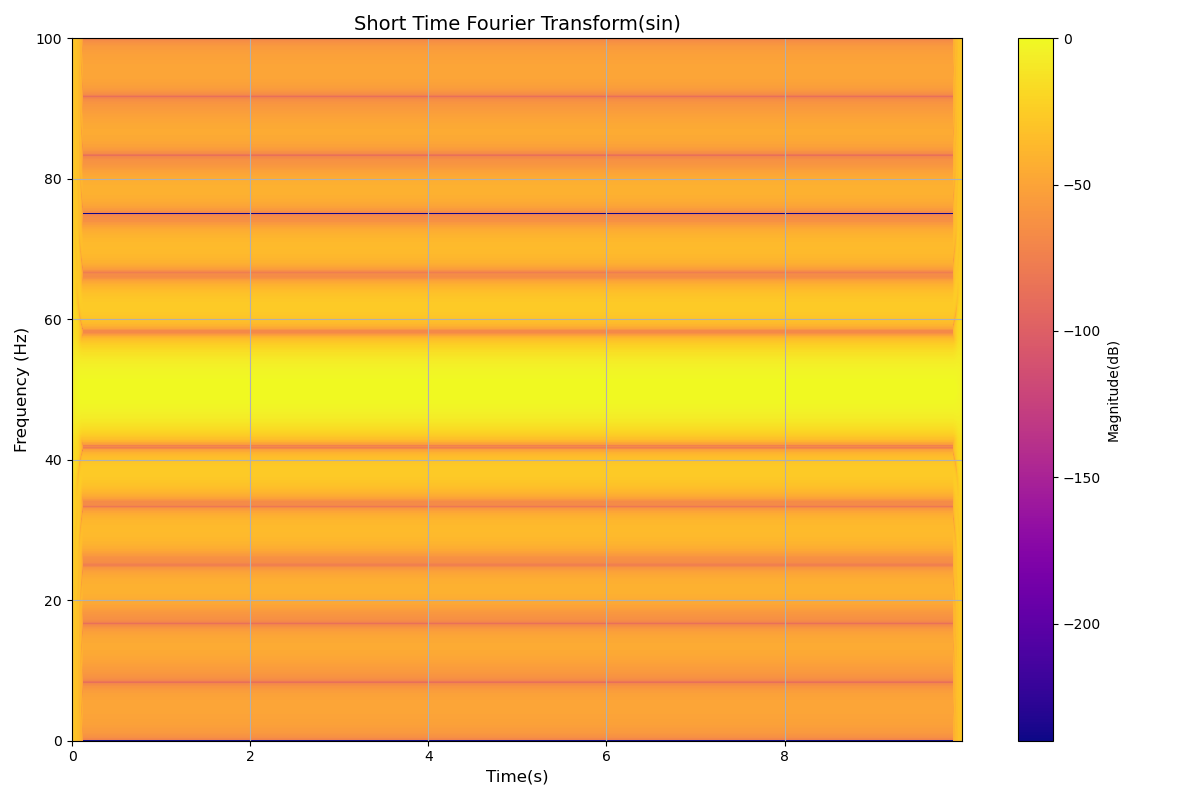
\includegraphics[scale = 0.35]{sin_1_50.0.png}
        \caption{STFT of $sin(w_ot)$ with Window Size 50 and overlap of 49(Bartlett Window)}
        \label{fig:1}
        \end{figure}

        \begin{figure}[H]
        \centering
        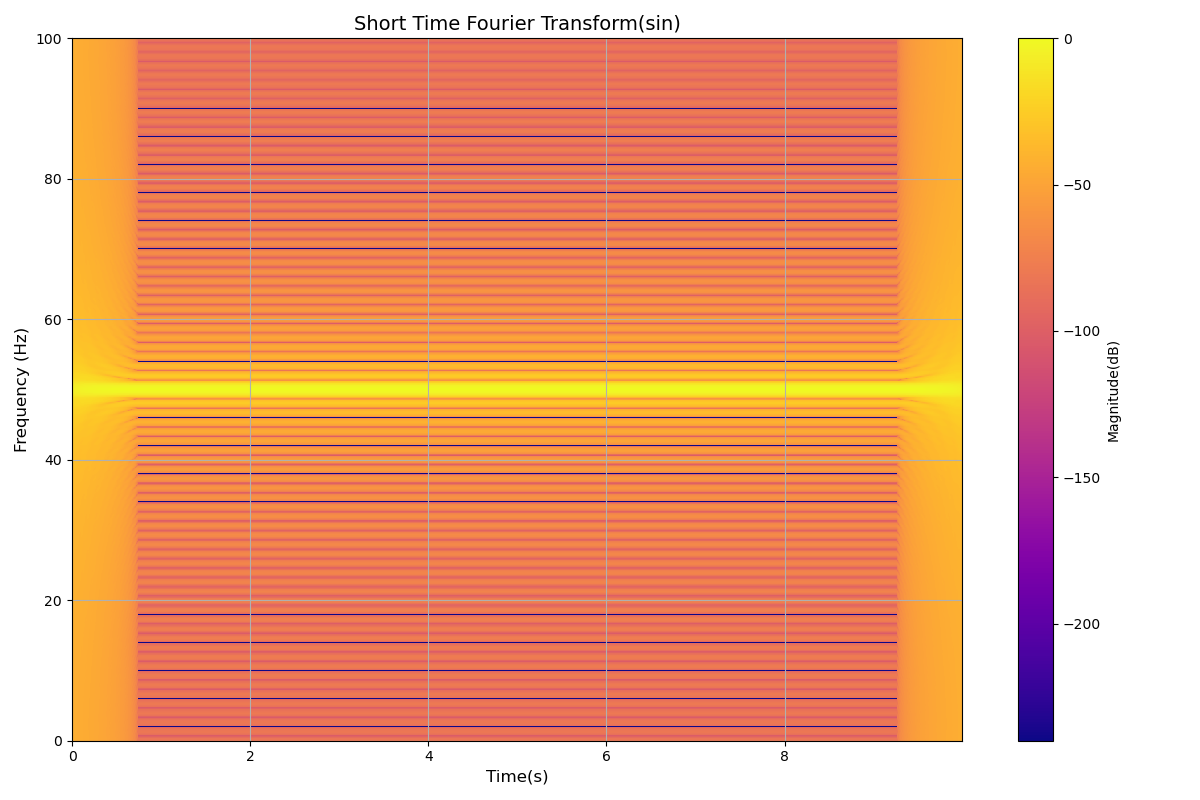
\includegraphics[scale = 0.35 ]{sin_1_300.0.png}
        \caption{STFT of $sin(w_ot)$ with Window Size 300 and overlap of 299(Bartlett Window)}
        \label{fig:2}
        \end{figure}

        \begin{figure}[H]
        \centering
        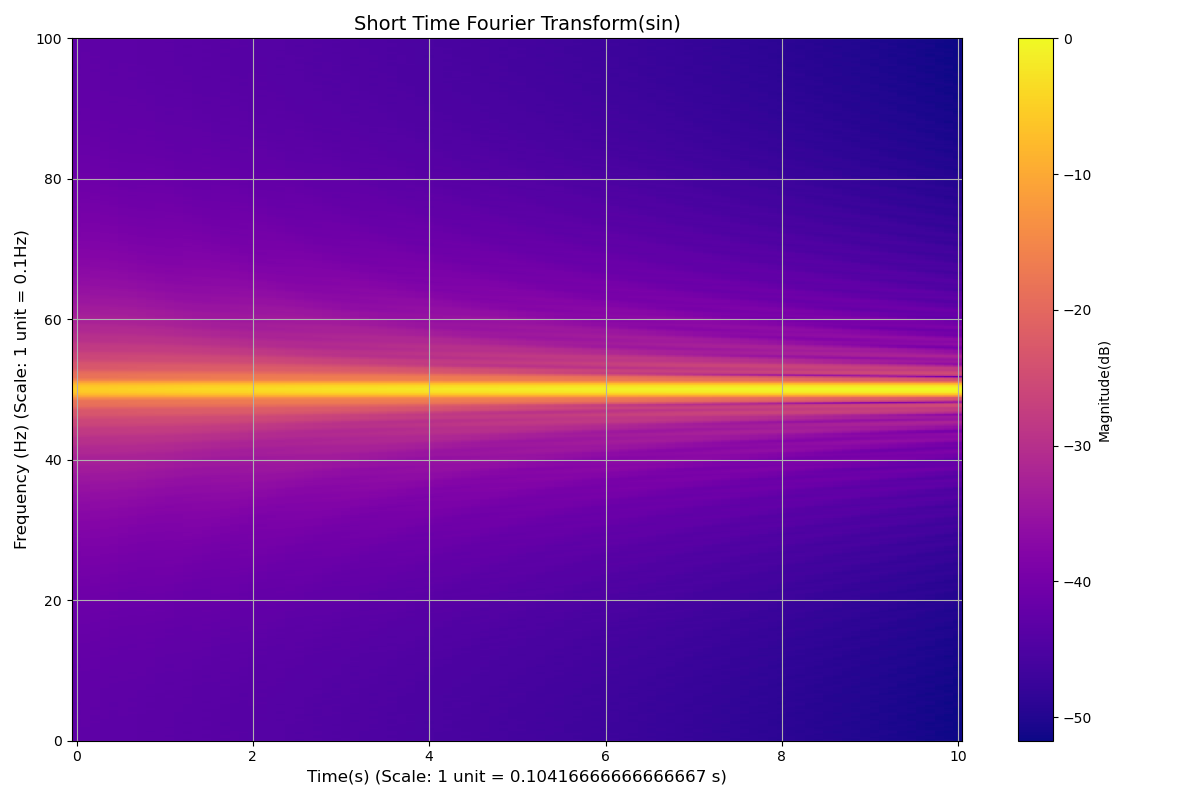
\includegraphics[scale = 0.35]{sin_21_300.0.png}
        \caption{STFT of $sin(w_ot)$ with Window Size 300 and overlap of 279(Bartlett Window)}
        \label{fig:3}
        \end{figure}
      
        \begin{itemize}
        
        \item[$\bullet$] $e^{-\frac{(x-5)^2}{\sigma^2}}$:\\
        Gaussian has a frequency of 0 almost all the time. The fourier transform of gaussian is a gaussian which has max frequency component near the center or zero frequency. Again, the similar pattern is seen, with more overlap there is many side lobe, that goes away when overlap is decreased. One important observation is that when the overlap is more, more information is retained. In the middle portion the spectrogram value is higher for frequency greater than 0. That should be the case because in the middle portion when multiplied by window function the function would not be exactly a straight line so there must be some magnitude at frequency above 0 and 0 for values near both ends. These information is lost when the overlap is reduced since almost whole of the signal has a 0 frequency over the whole time interval. Fig.\ref{fig:4} shows the plot with poor frequency resolution. It seems as if there are multiple frequencies present. Fig.\ref{fig:5} shows the plot with better frequency resolution but with side lobes. Fig.\ref{fig:6} shows the plot where side lobes are absent but it seems all the time the function has a frequency 0. 
        
        \end{itemize}

        \begin{figure}[H]
        \centering
        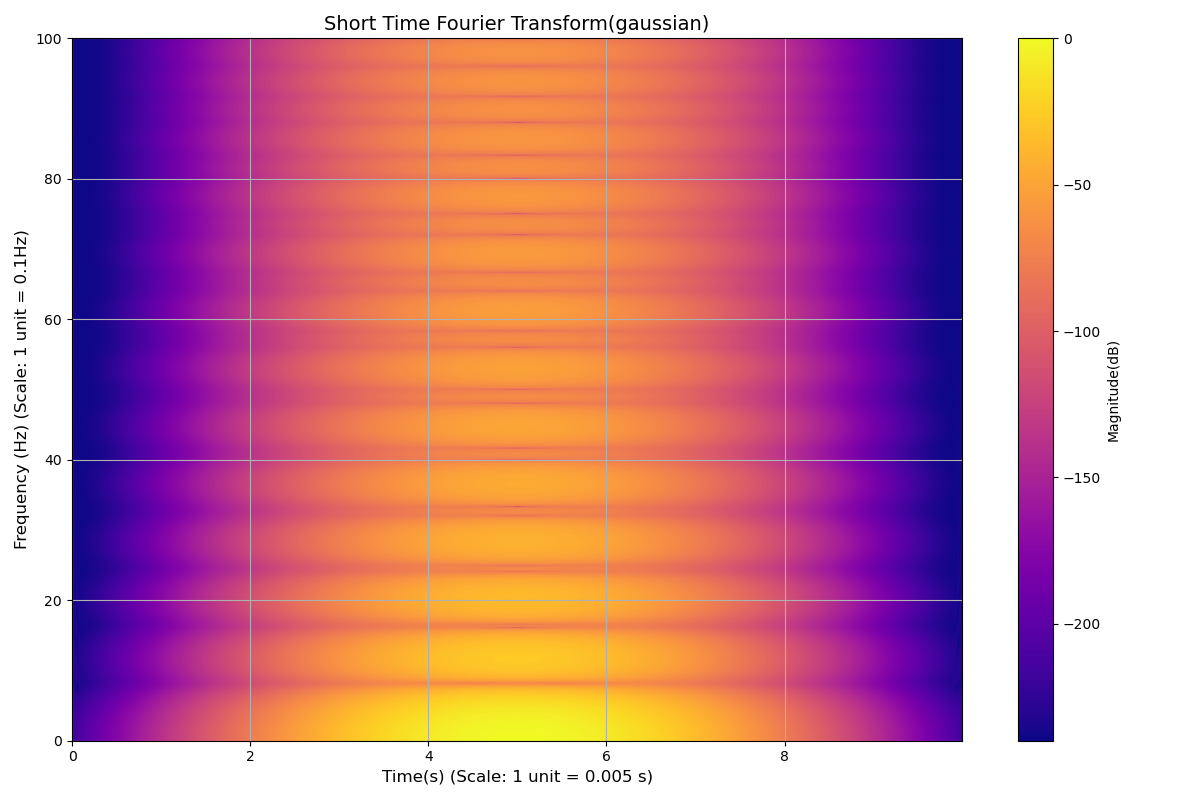
\includegraphics[scale = 0.35]{gaussian_1_50.0.png}
        \caption{STFT of $e^{-\frac{(x-5)^2}{\sigma^2}}$ with Window Size 50 and overlap of 49(Bartlett Window)}
        \label{fig:4}
        \end{figure}

        \begin{figure}[H]
        \centering
        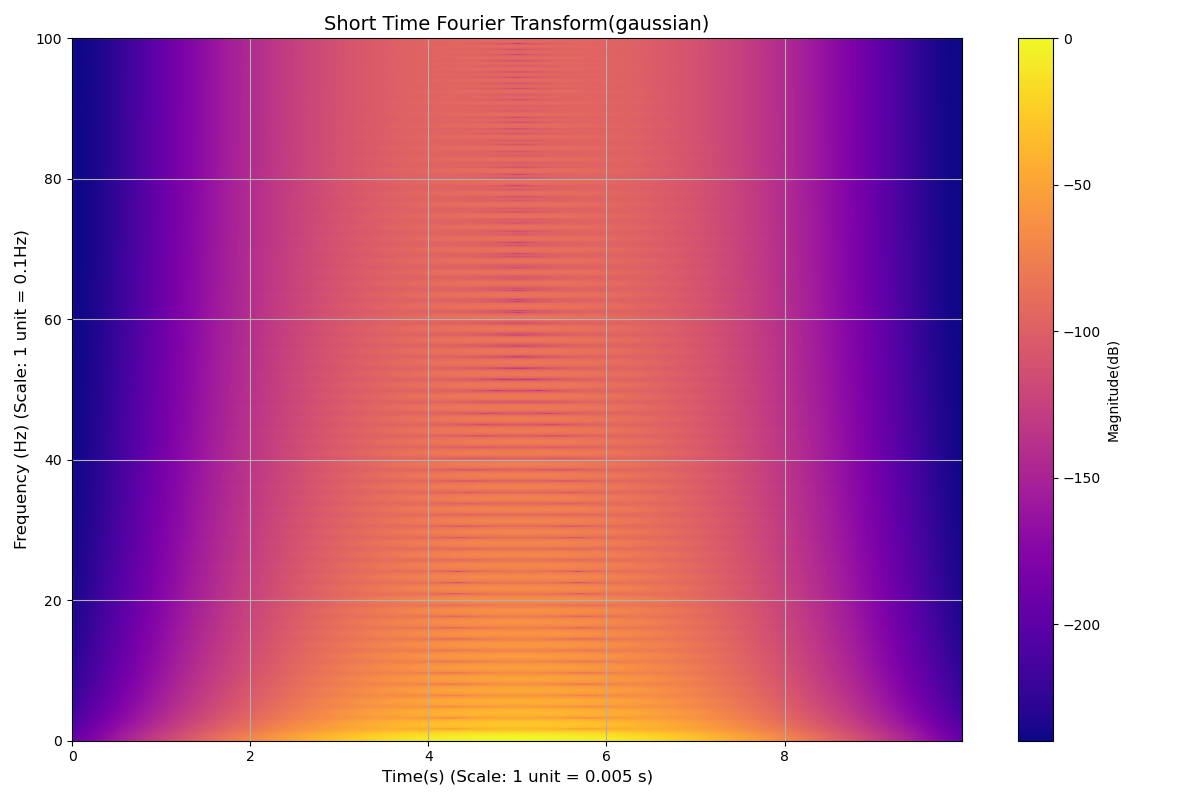
\includegraphics[scale = 0.35 ]{gaussian_1_250.0.png}
        \caption{STFT of $e^{-\frac{(x-5)^2}{\sigma^2}}$ with Window Size 250 and overlap of 249(Bartlett Window)}
        \label{fig:5}
        \end{figure}

        \begin{figure}[H]
        \centering
        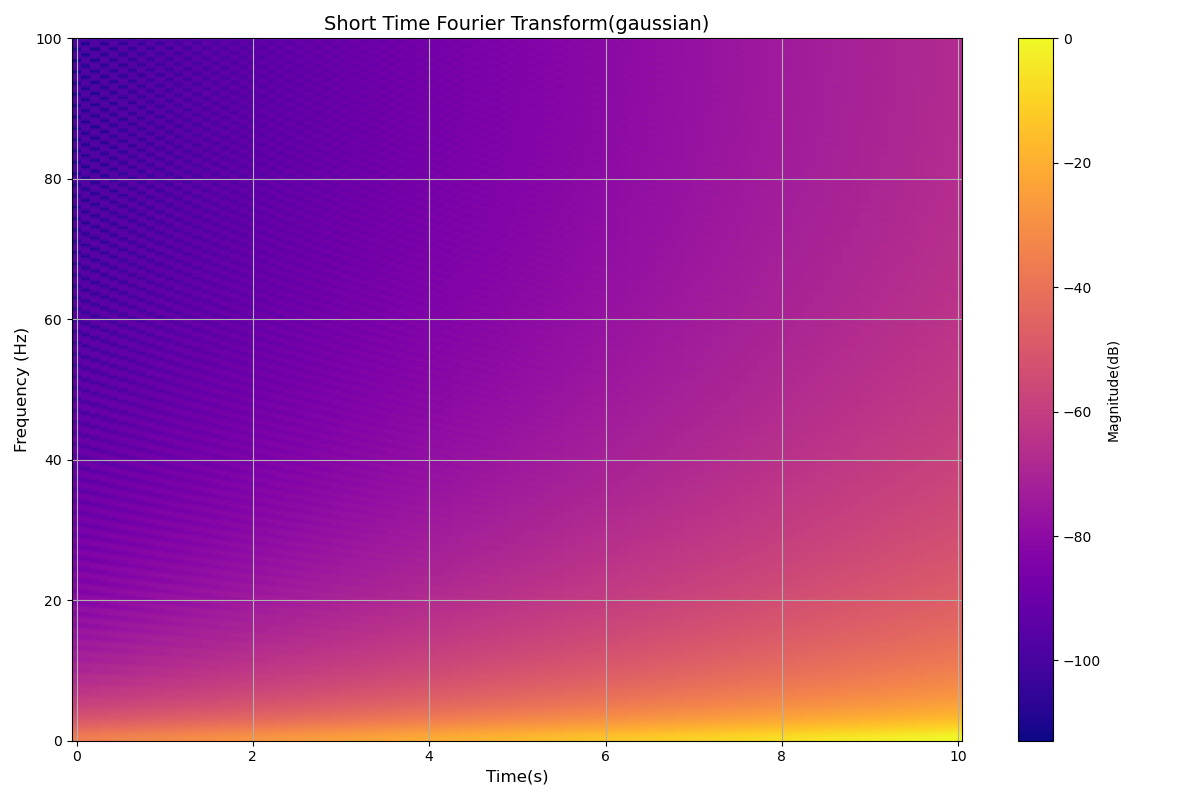
\includegraphics[scale = 0.35]{gaussian_21_250.0.png}
        \caption{STFT of $e^{-\frac{(x-5)^2}{\sigma^2}}$ with Window Size 250 and overlap of 229(Bartlett Window)}
        \label{fig:6}
        \end{figure}
      
      \begin{itemize}

      \item[$\bullet$] $sin(2\pi\gamma(t)t)$, where $\gamma(t)$ varies linearly between $5Hz$ and $50Hz$: \\
      This was a interesting problem. When there was maximum overlap, the linear chirp is clearly visible to be increasing from $5Hz$ to $50Hz$. The resolution was poor for Fig.\ref{fig:7} the frequency improved by increasing the time domain window in Fig.\ref{fig:8} .But when we change the overlap to be less than that. Then we loose all the information about the variation of the frequency and we almost get the lower frequency signal in the plot, just as in Fig.\ref{fig:9}

      \end{itemize}
      \begin{itemize}
      \item[$\bullet$] $e^{-\frac{(x-5)^2}{\sigma^2}}sin(w_0t)$, $0 \leq t < 10$: \\
      This has almost the same graph and observation as the normal gaussian function. The frequency content is different since it is multiplied by a constant frequency term of $sin$. So the net frequency content is around $50Hz$ not $0$. Fig.\ref{fig:10} gives the short time fourier transform of the signal with poor frequency. Fig.\ref{fig:11} gives the finer resolution one. Fig.\ref{fig:12} gives the function with less overlap. An interesting observation is the presence of horizontal lines throughout the time axis. When the sin is multiplied by the gaussian function at low values, it fluctuates rapidly between positive and negative, introducing impulse-like components that contain all frequencies, appearing as vertical lines.
      \end{itemize}

        \begin{figure}[H]
        \centering
        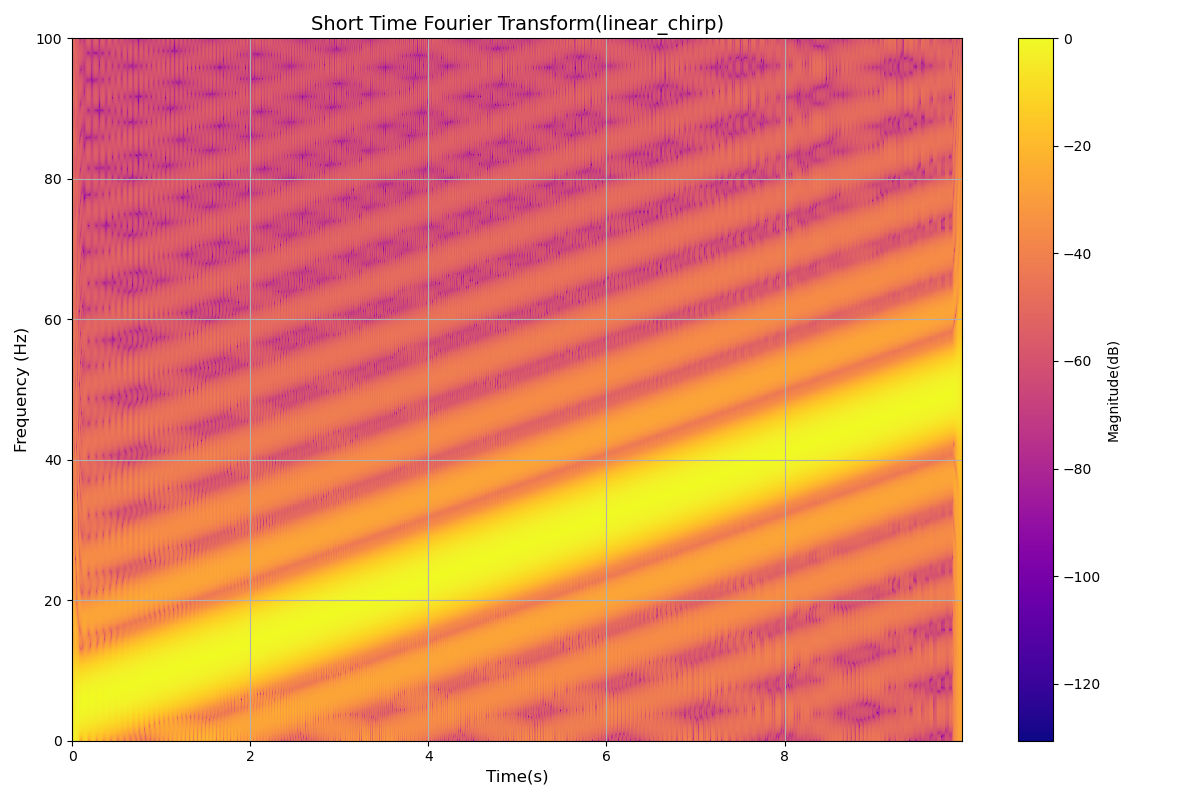
\includegraphics[scale = 0.35]{linear_chirp_1_50.0.png}
        \caption{STFT of $sin(2\pi\gamma(t)t)$ with Window Size 50 and overlap of 49(Bartlett Window)}
        \label{fig:7}
        \end{figure}

        \begin{figure}[H]
        \centering
        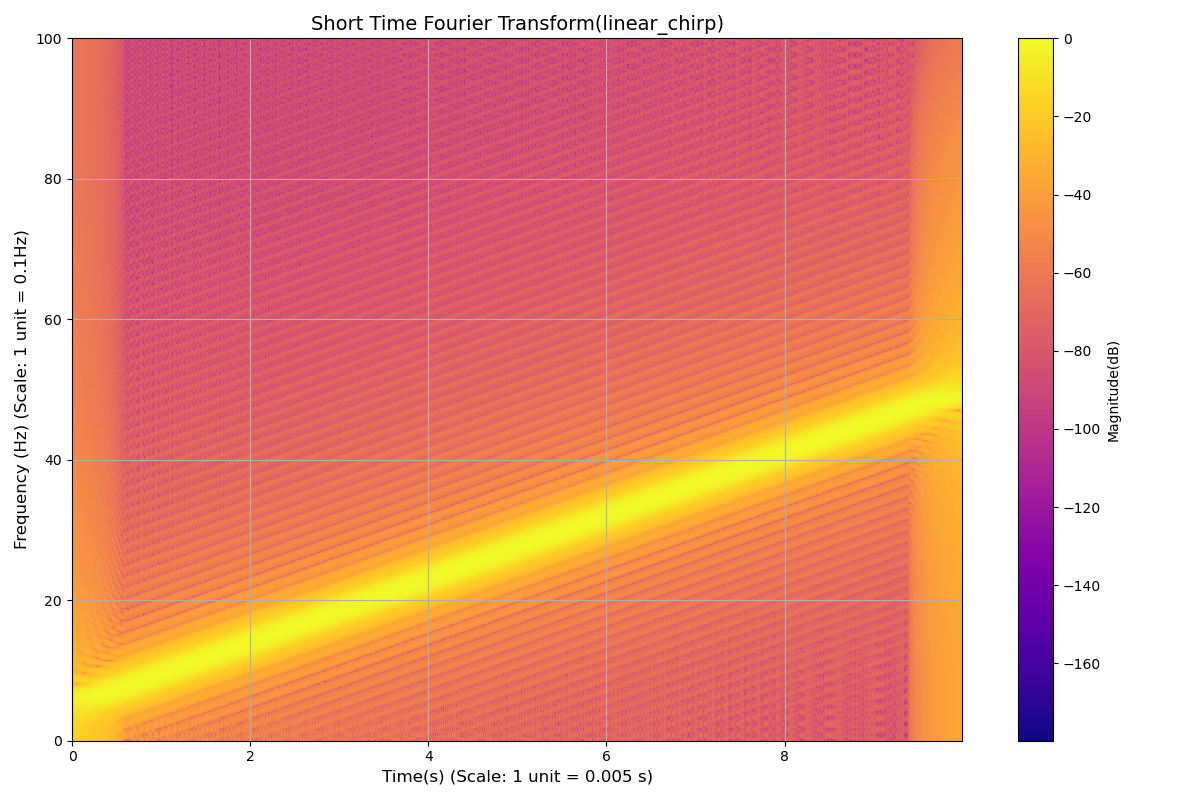
\includegraphics[scale = 0.35 ]{linear_chirp_1_250.0.png}
        \caption{STFT of $sin(2\pi\gamma(t)t)$ with Window Size 250 and overlap of 249(Bartlett Window)}
        \label{fig:8}
        \end{figure}

        \begin{figure}[H]
        \centering
        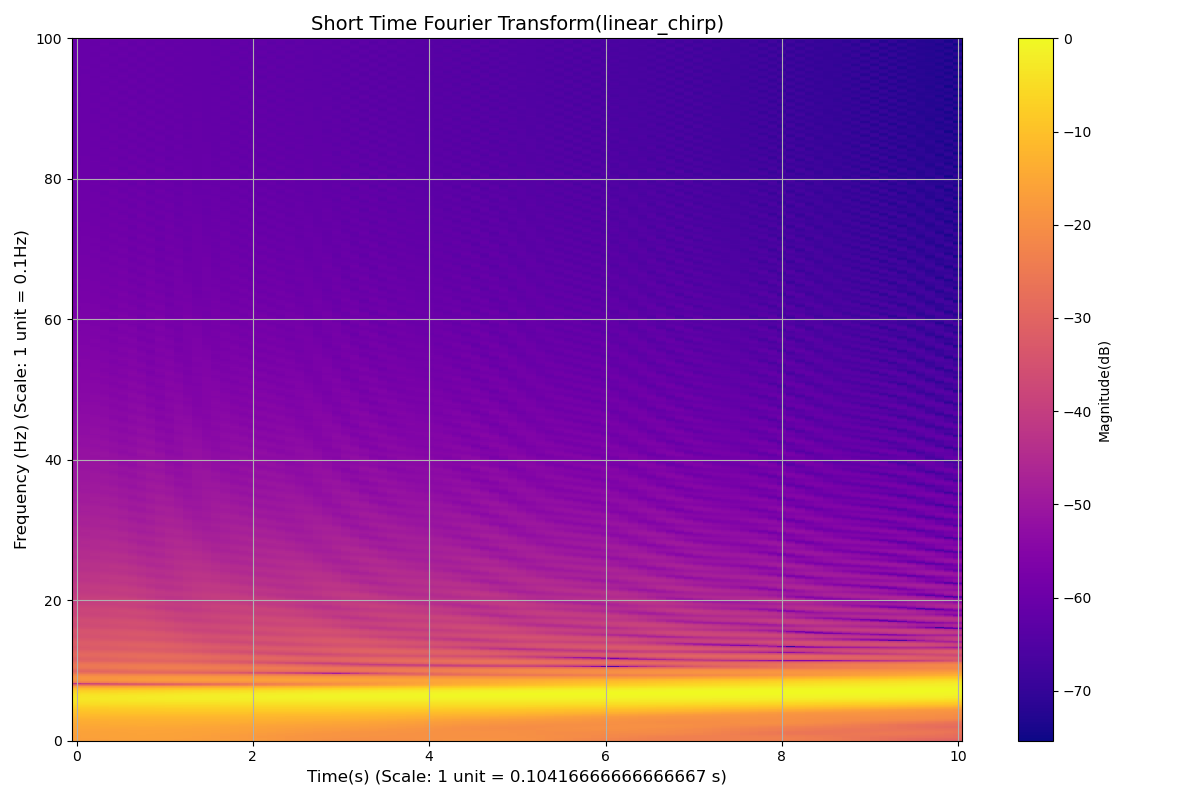
\includegraphics[scale = 0.35]{linear_chirp_21_250.0.png}
        \caption{STFT of $sin(2\pi\gamma(t)t)$  with Window Size 250 and overlap of 229(Bartlett Window)}
        \label{fig:9}
        \end{figure}

      
        \begin{figure}[H]
        \centering
        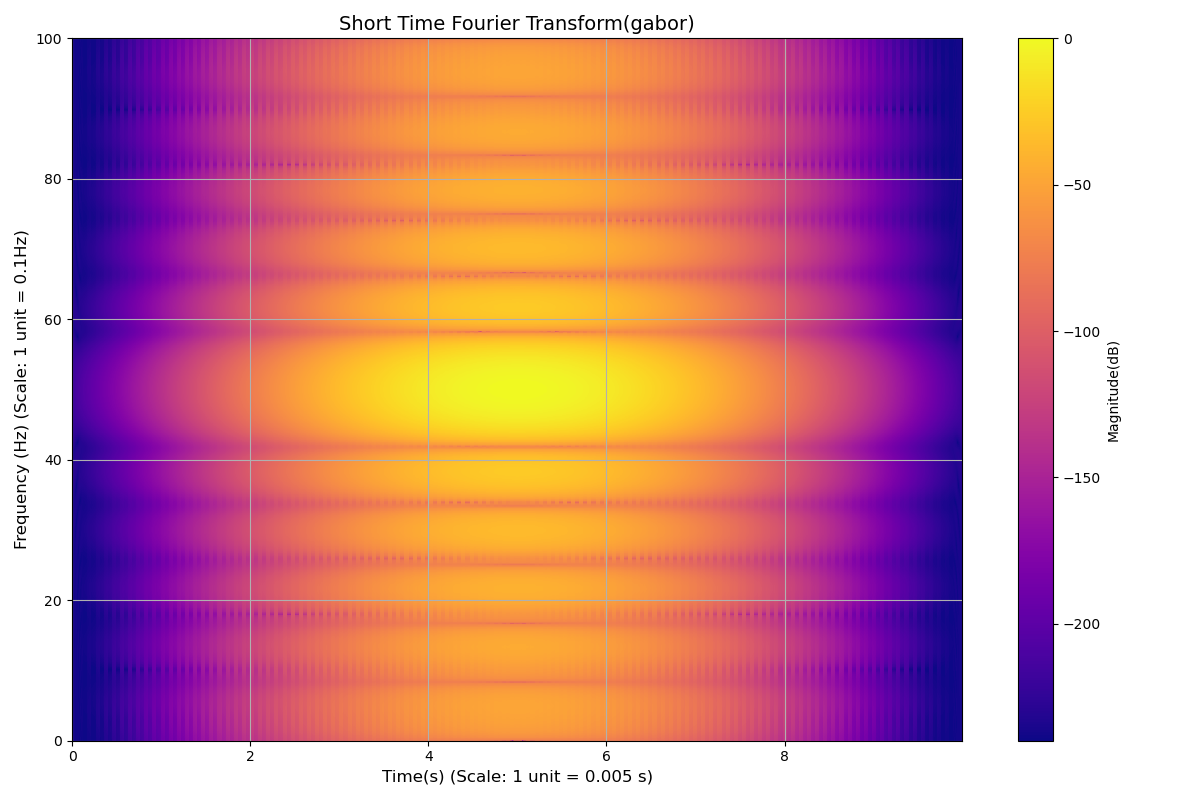
\includegraphics[scale = 0.35]{gabor_1_50.0.png}
        \caption{STFT of $e^{-\frac{(x-5)^2}{\sigma^2}}sin(w_0t)$ with Window Size 50 and overlap of 49(Bartlett Window)}
        \label{fig:10}
        \end{figure}

        \begin{figure}[H]
        \centering
        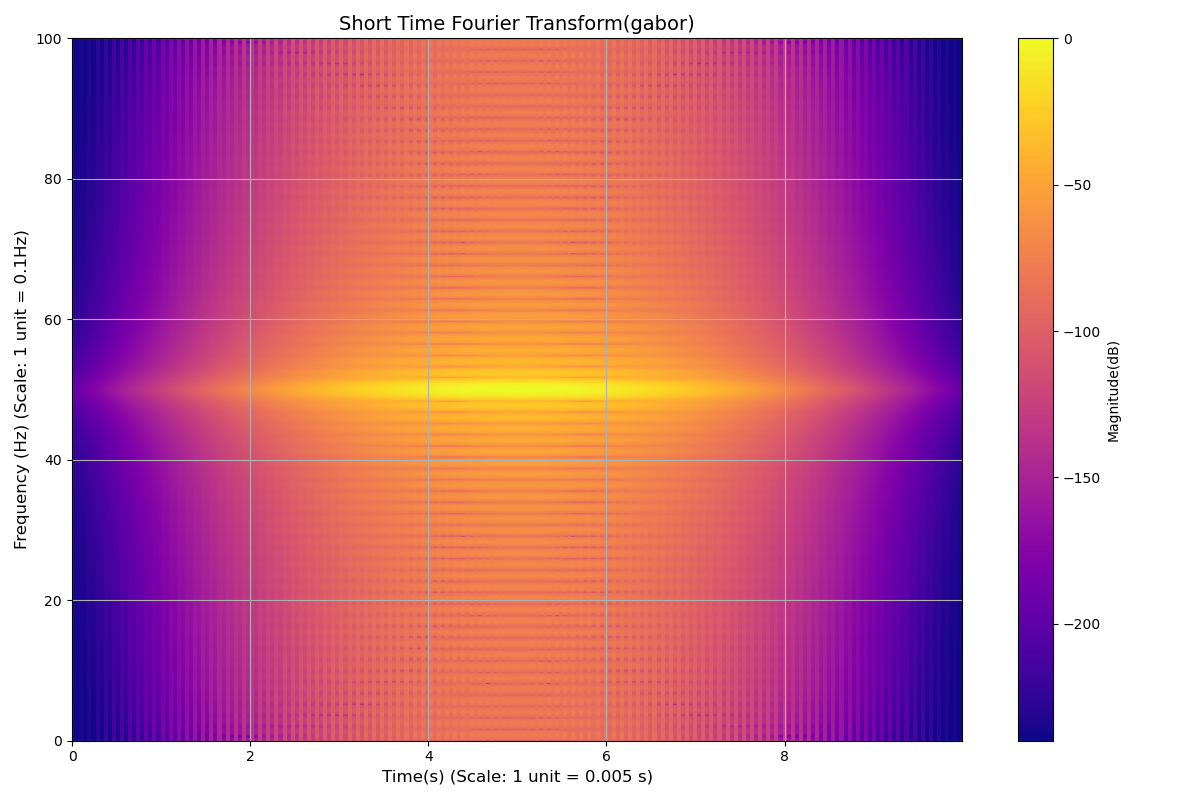
\includegraphics[scale = 0.35]{gabor_1_250.0.png}
        \caption{STFT of $e^{-\frac{(x-5)^2}{\sigma^2}}sin(w_0t)$ with Window Size 250 and overlap of 249(Bartlett Window)}
        \label{fig:11}
        \end{figure}

        \begin{figure}[H]
        \centering
        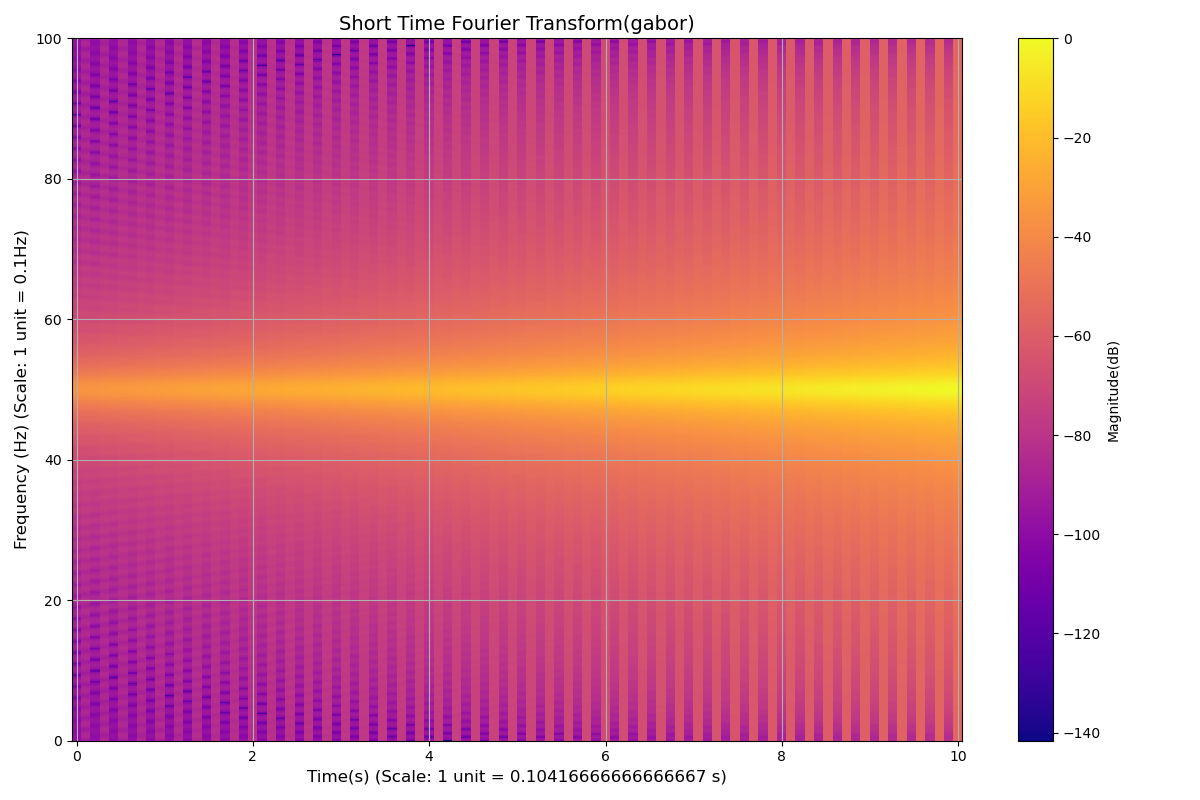
\includegraphics[scale = 0.35]{gabor_21_250.0.png}
        \caption{STFT of $e^{-\frac{(x-5)^2}{\sigma^2}}sin(w_0t)$ with Window Size 250 and overlap of 229(Bartlett Window)}
        \label{fig:12}
        \end{figure}

    \item[(ii)] \textbf{Gaussian Window:}
    The general observation for window length remained the same for the Gaussian Window also. But in general Gaussian Window has infinite support, and for creating the windows the signal was cut using a box function. So the properties of box also comes to play not only Gaussian Window. The Gaussian window was used with a standard deviation of 10 and with varying window. In general the frequency resolution was poorer than Bartlett. With less overlap almost in all the cases, useful information is lost as would be evident from the plots. 

    \begin{itemize}
      \item[$\bullet$] $sin(w_ot)$:
    \end{itemize}
        \begin{figure}[H]
        \centering
        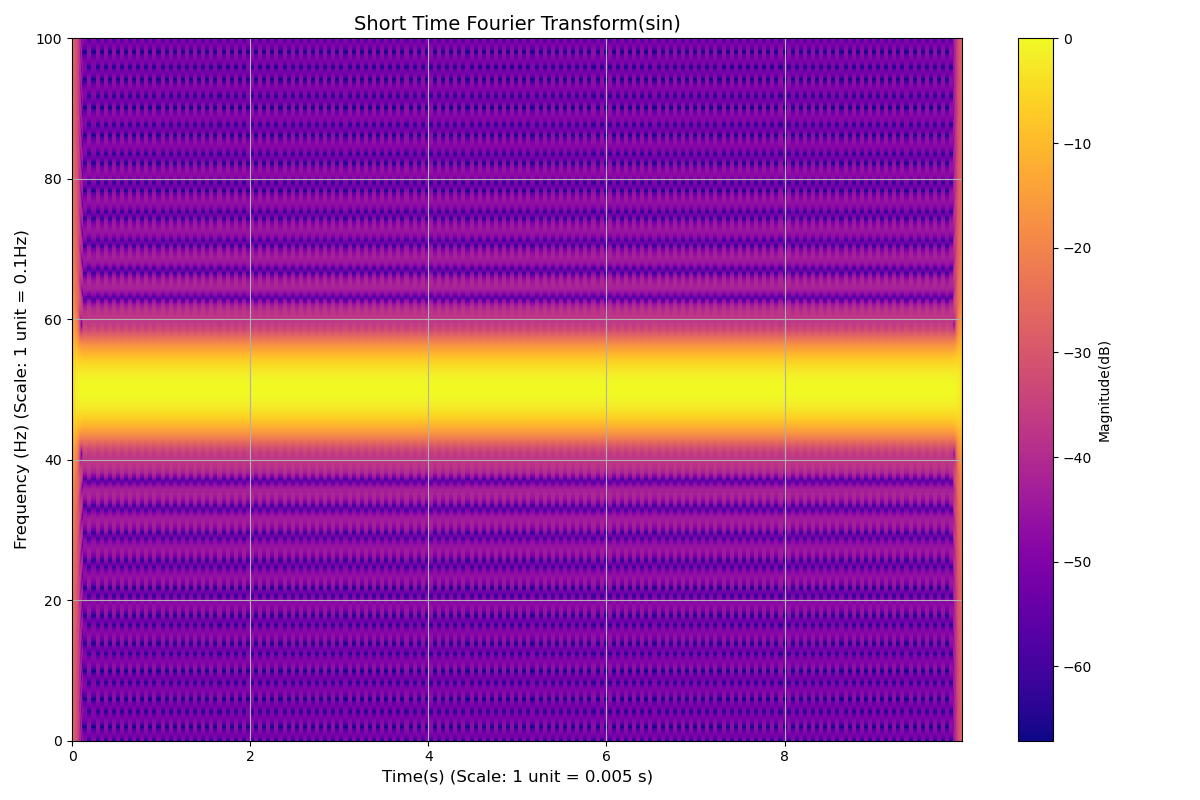
\includegraphics[scale = 0.35]{Gau_Win_sin_1_50.0.png}
        \caption{STFT of $sin(w_ot)$ with Window Size 50 and overlap of 49(Gaussian Window)}
        \label{fig:13}
        \end{figure}

        \begin{figure}[H]
        \centering
        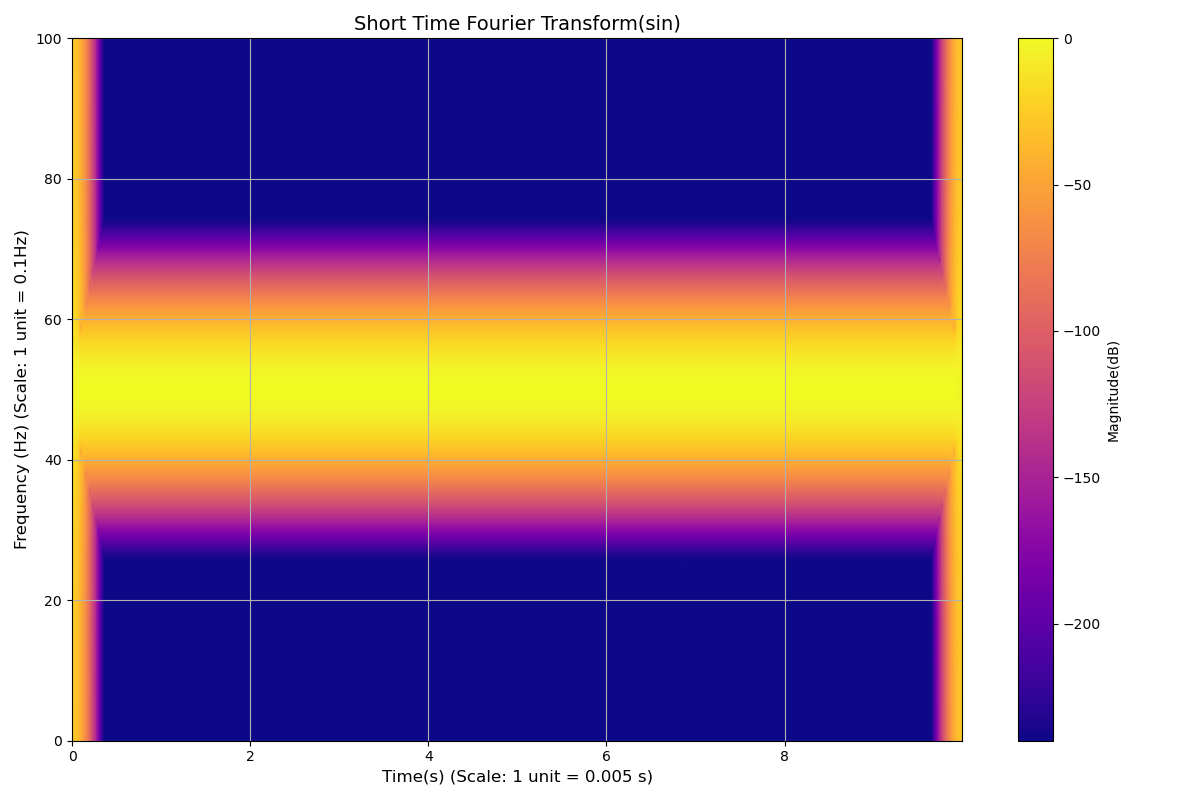
\includegraphics[scale = 0.35]{Gau_Win_sin_1_250.0.png}
        \caption{STFT of $sin(w_ot)$ with Window Size 250 and overlap of 249(Gaussian Window)}
        \label{fig:14}
        \end{figure}

        \begin{figure}[H]
        \centering
        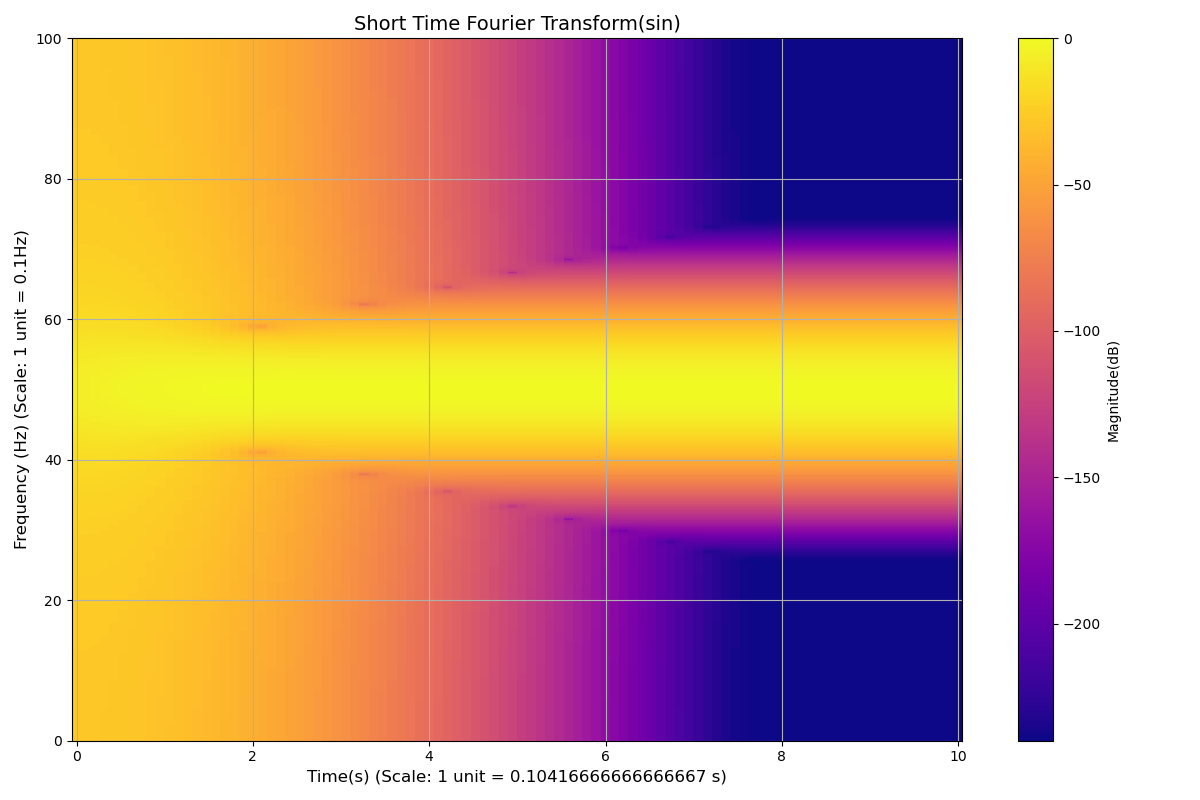
\includegraphics[scale = 0.35]{Gau_Win_sin_21_250.0.png}
        \caption{STFT of $sin(w_ot)$ with Window Size 250 and overlap of 229(Gaussian Window)}
        \label{fig:15}
        \end{figure}
    \begin{itemize}
      \item[$\bullet$] $e^{-\frac{(x-5)^2}{\sigma^2}}$:
    \end{itemize}

        \begin{figure}[H]
        \centering
        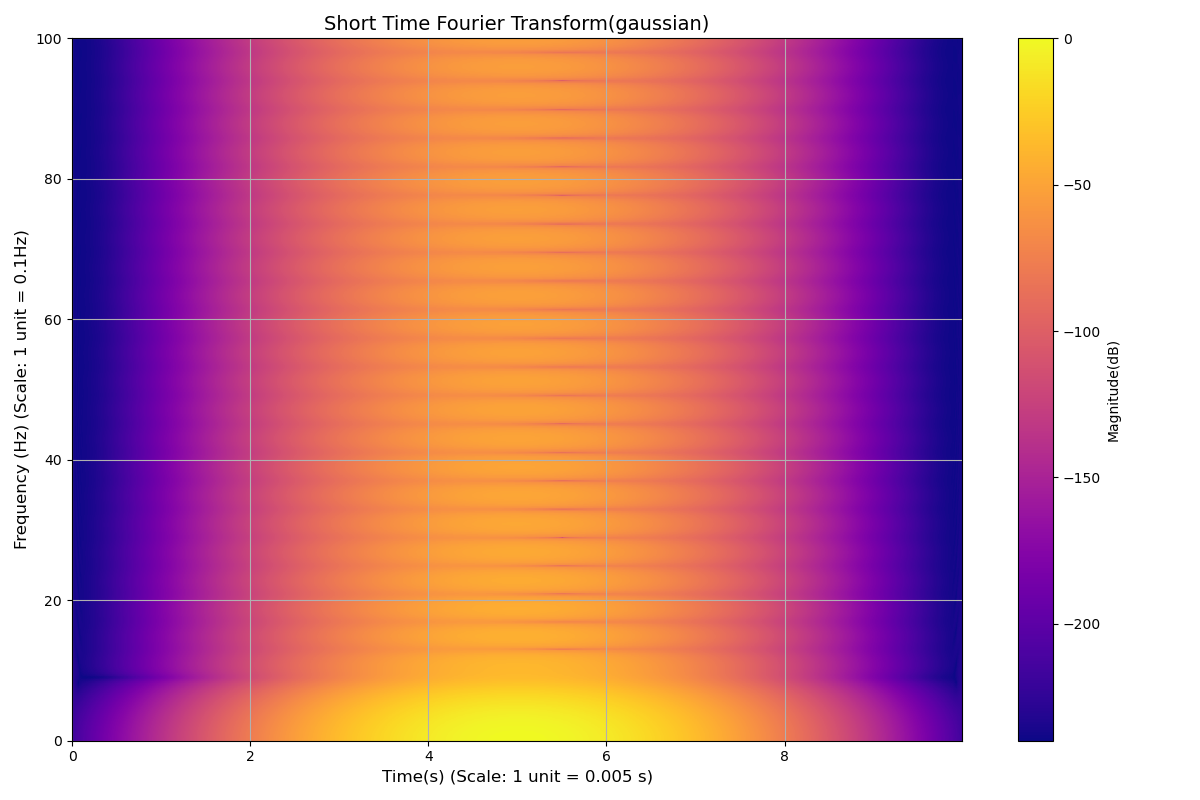
\includegraphics[scale = 0.35]{Gau_Win_gaussian_1_50.0.png}
        \caption{STFT of $e^{-\frac{(x-5)^2}{\sigma^2}}$ with Window Size 50 and overlap of 49(Gaussian Window)}
        \label{fig:16}
        \end{figure}

        \begin{figure}[H]
        \centering
        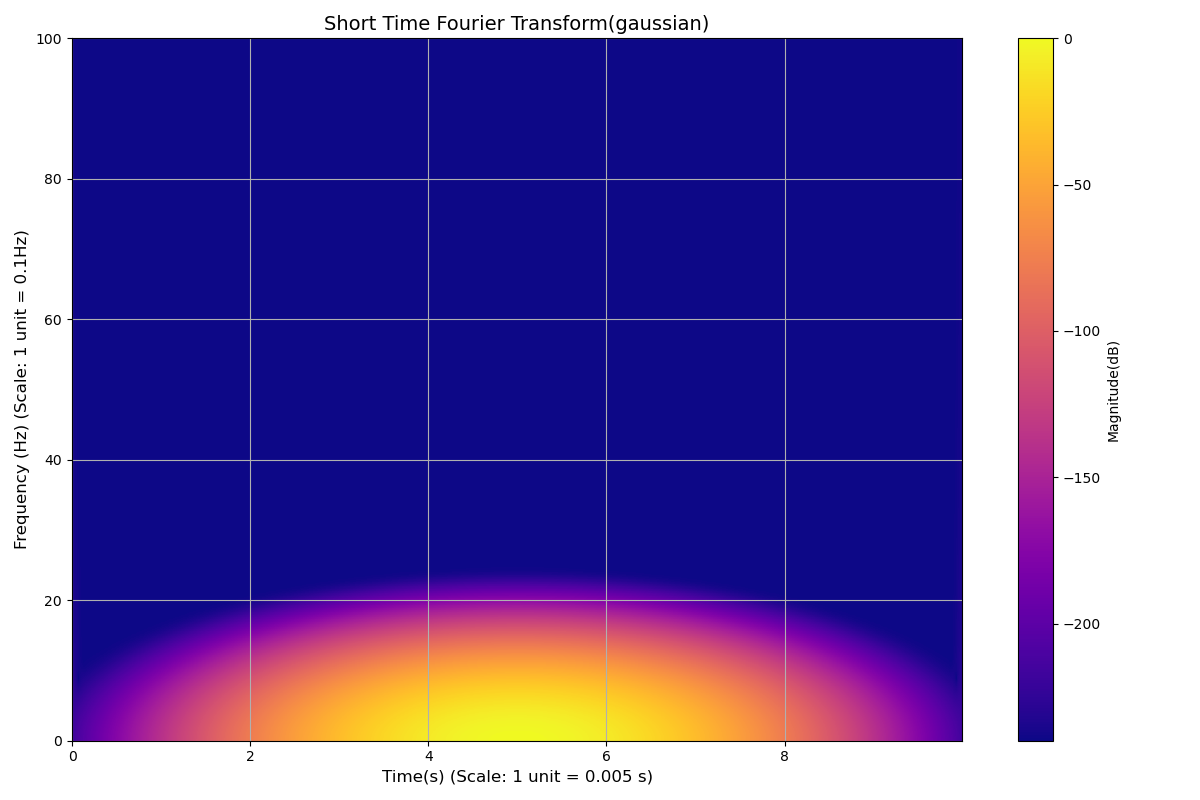
\includegraphics[scale = 0.35 ]{Gau_Win_gaussian_1_250.0.png}
        \caption{STFT of $e^{-\frac{(x-5)^2}{\sigma^2}}$ with Window Size 250 and overlap of 249(Gaussian Window)}
        \label{fig:17}
        \end{figure}

        \begin{figure}[H]
        \centering
        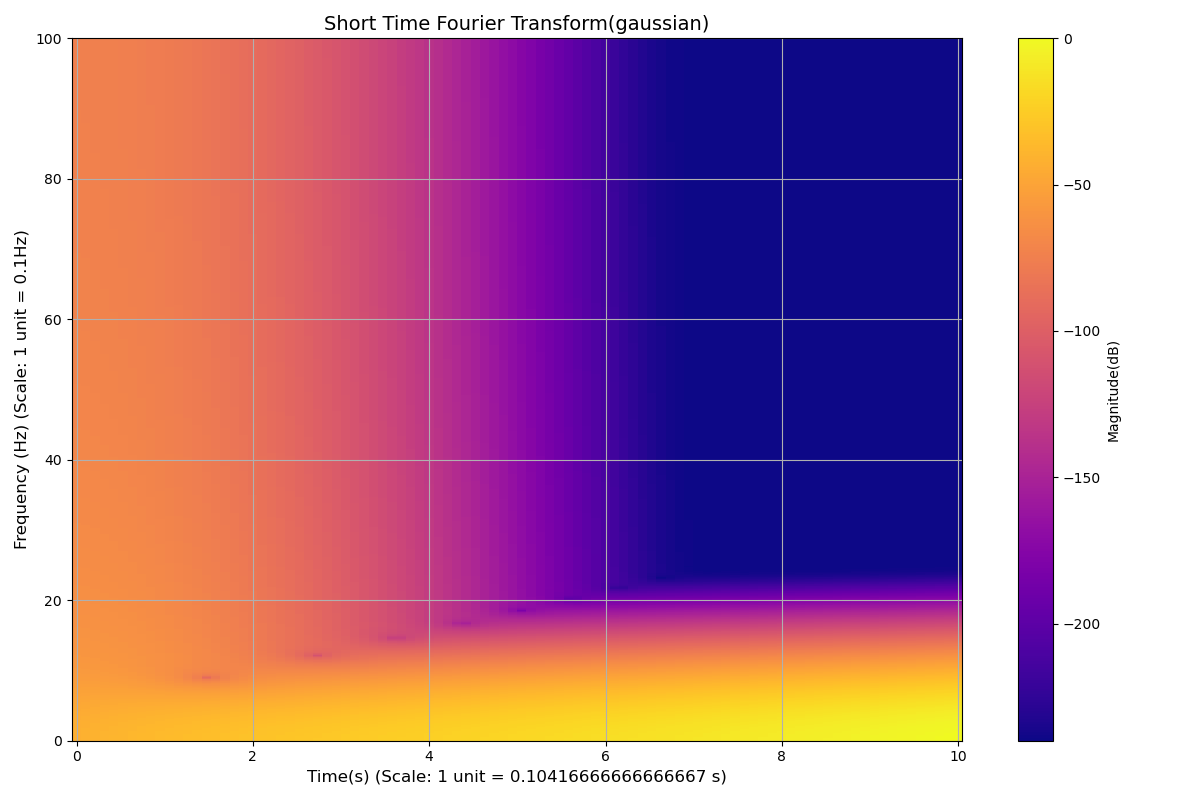
\includegraphics[scale = 0.35]{Gau_Win_gaussian_21_250.0.png}
        \caption{STFT of $e^{-\frac{(x-5)^2}{\sigma^2}}$ with Window Size 250 and overlap of 229(Gaussian Window)}
        \label{fig:18}
        \end{figure}

      \begin{itemize}
         \item[$\bullet$] $sin(2\pi\gamma(t)t)$, where $\gamma(t)$ varies linearly between $5Hz$ and $50Hz$:
      \end{itemize}
        
        \begin{figure}[H]
        \centering
        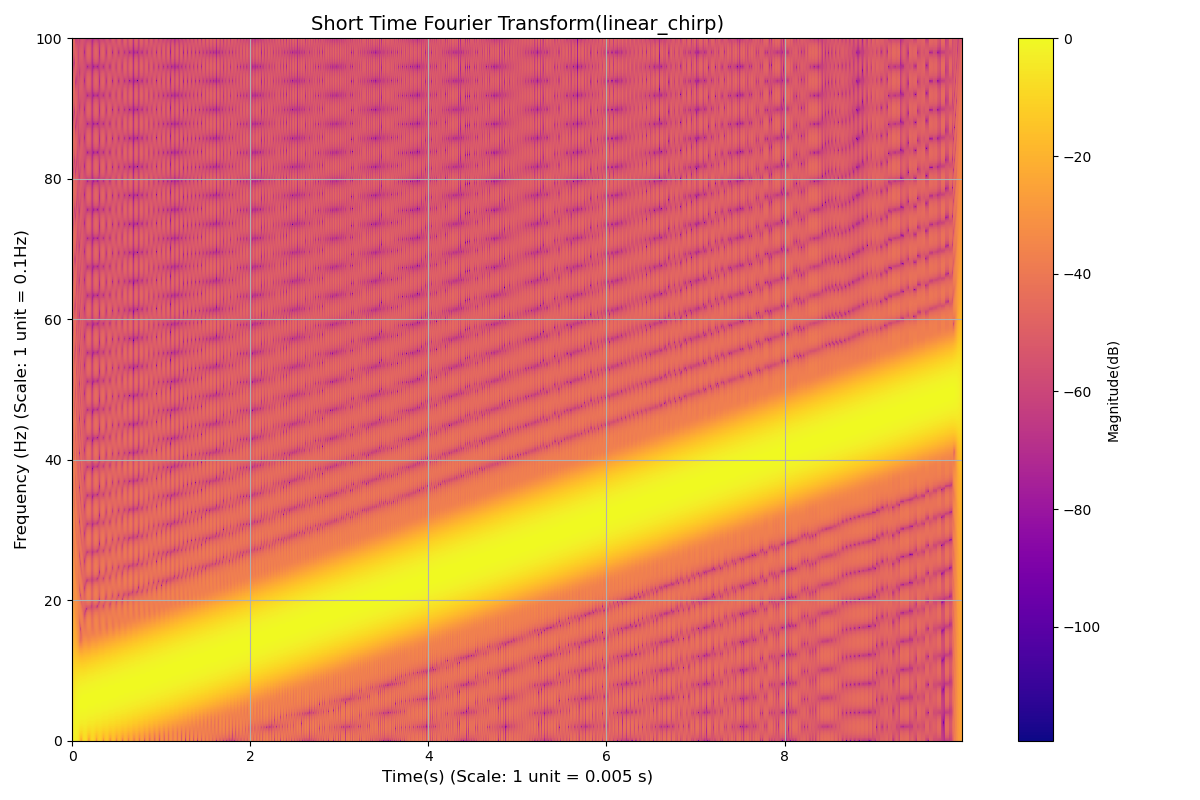
\includegraphics[scale = 0.35]{Gau_Win_linear_chirp_1_50.0.png}
        \caption{STFT of $sin(2\pi\gamma(t)t)$ with Window Size 50 and overlap of 49(Gaussian Window)}
        \label{fig:19}
        \end{figure}

        \begin{figure}[H]
        \centering
        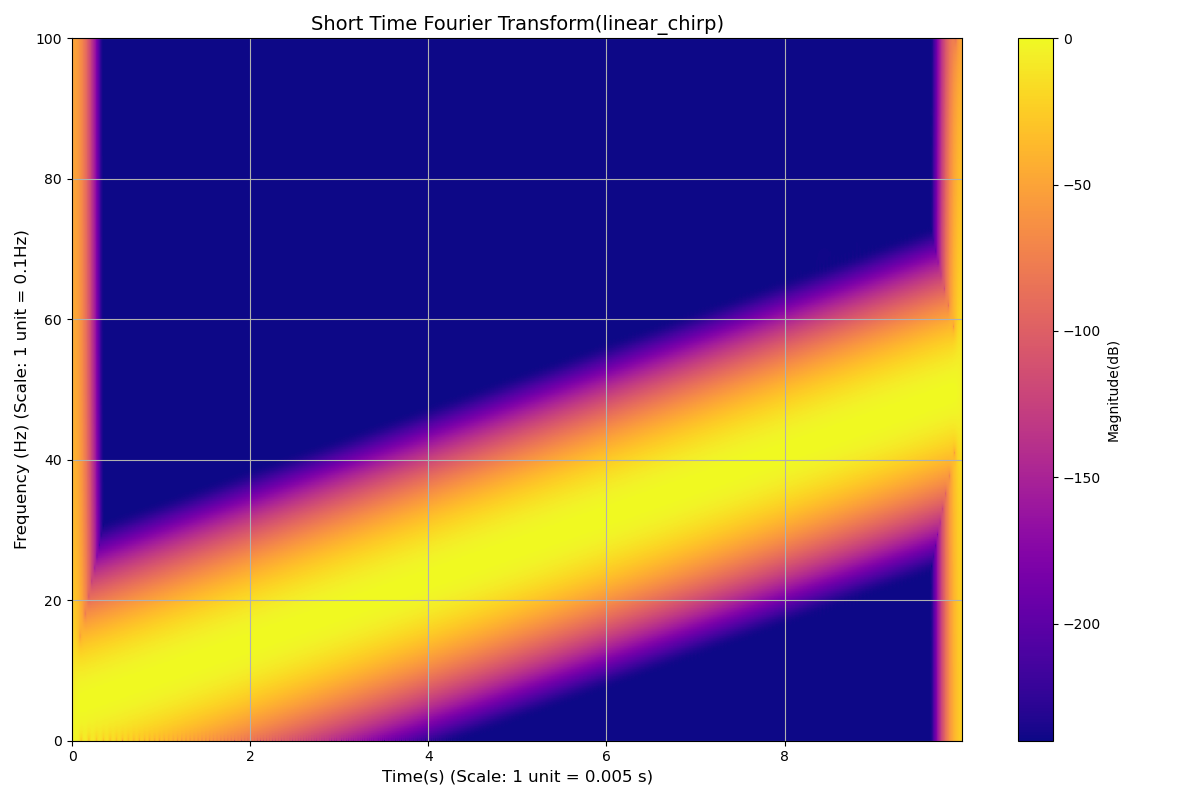
\includegraphics[scale = 0.35 ]{Gau_Win_linear_chirp_1_250.0.png}
        \caption{STFT of $sin(2\pi\gamma(t)t)$ with Window Size 250 and overlap of 249(Gaussian Window)}
        \label{fig:20}
        \end{figure}

        \begin{figure}[H]
        \centering
        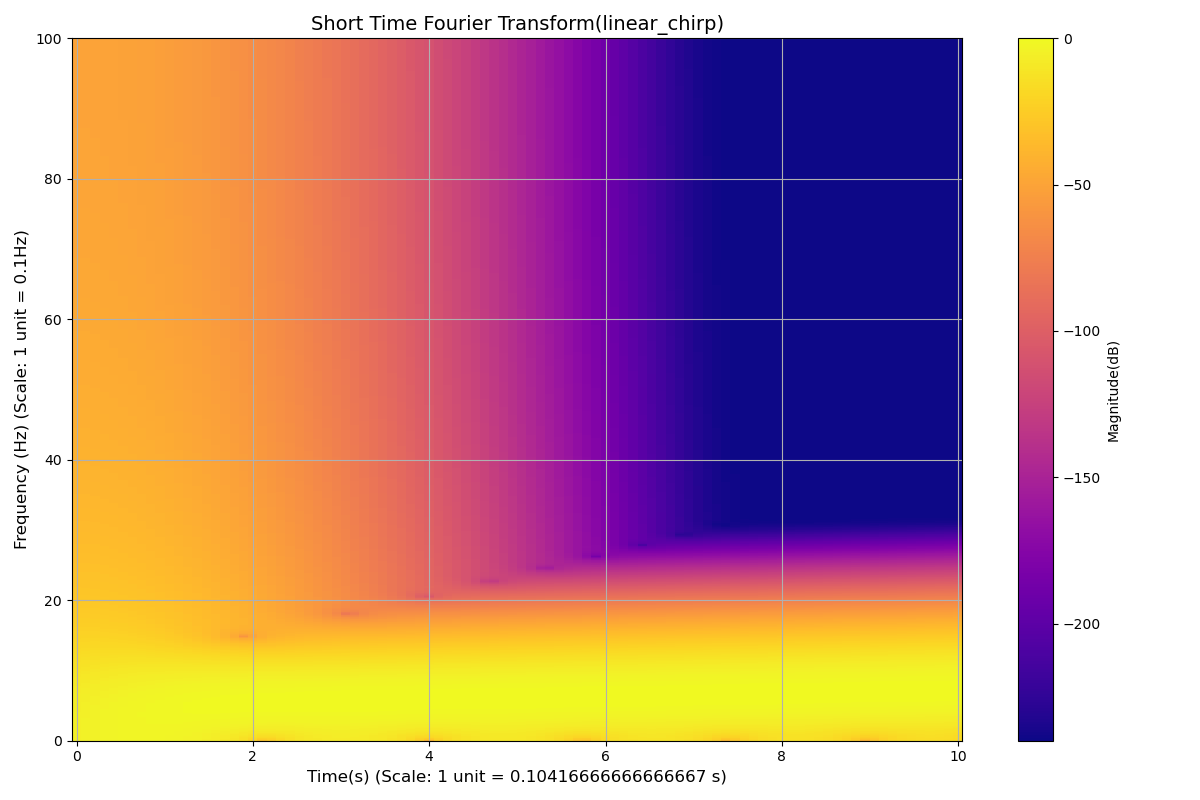
\includegraphics[scale = 0.35]{Gau_Win_linear_chirp_21_250.0.png}
        \caption{STFT of $sin(2\pi\gamma(t)t)$  with Window Size 250 and overlap of 229(Gaussian Window)}
        \label{fig:21}
        \end{figure}

      \begin{itemize}
        \item[$\bullet$] $e^{-\frac{(x-5)^2}{\sigma^2}}sin(w_0t)$, $0 \leq t < 10$:
      \end{itemize}
      
        \begin{figure}[H]
        \centering
        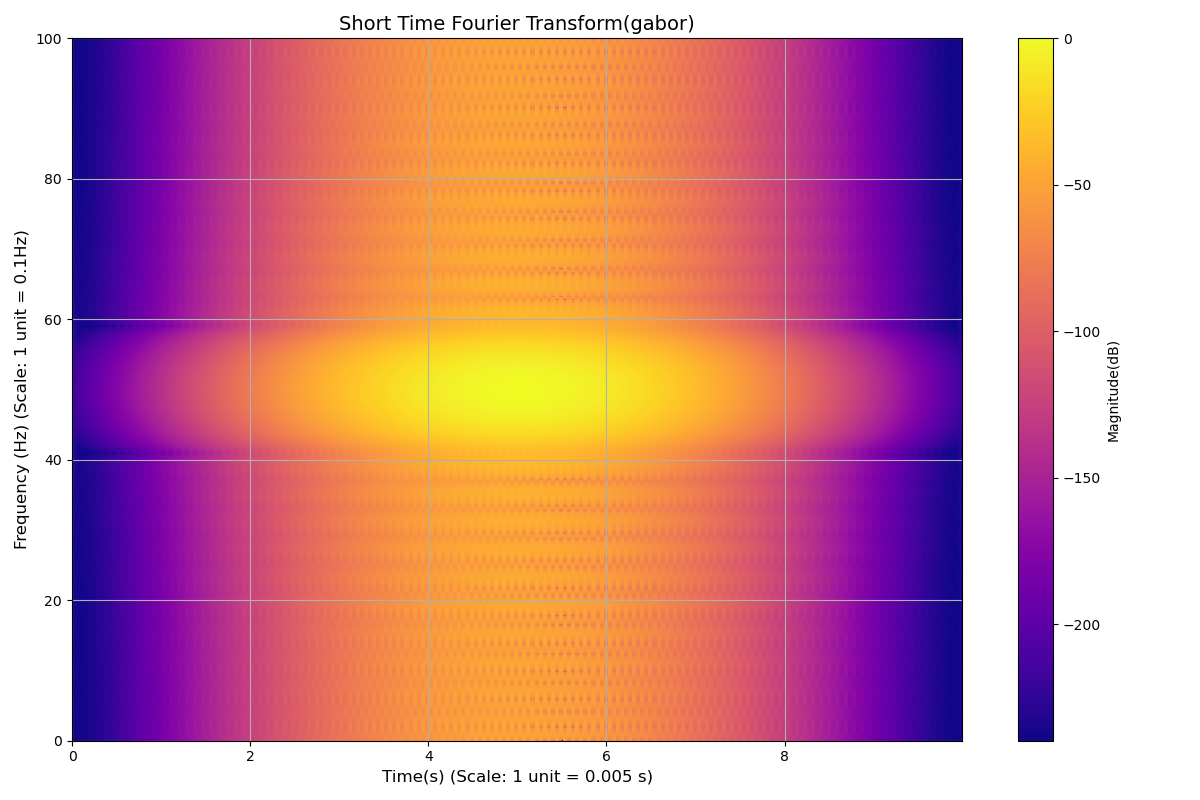
\includegraphics[scale = 0.35]{Gau_Win_gabor_1_50.0.png}
        \caption{STFT of $e^{-\frac{(x-5)^2}{\sigma^2}}sin(w_0t)$ with Window Size 50 and overlap of 49(Gaussian Window)}
        \label{fig:22}
        \end{figure}

        \begin{figure}[H]
        \centering
        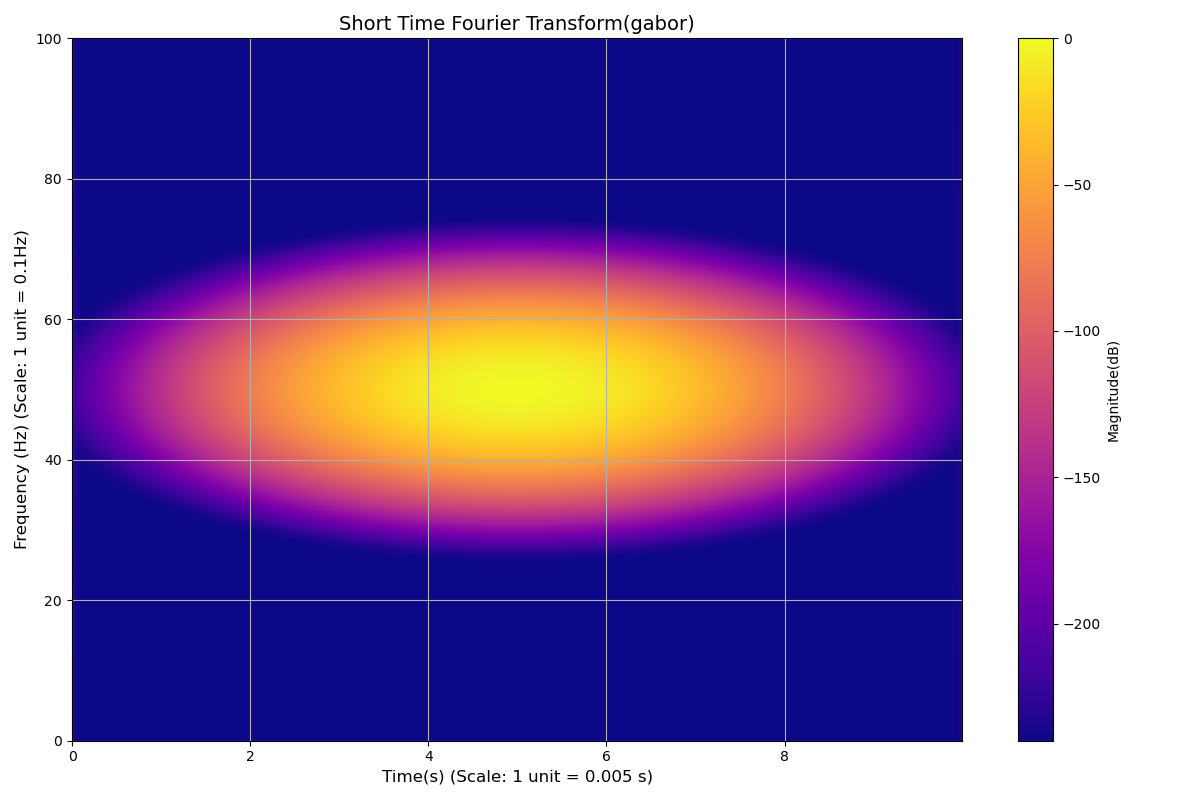
\includegraphics[scale = 0.35]{Gau_Win_gabor_1_250.0.png}
        \caption{STFT of $e^{-\frac{(x-5)^2}{\sigma^2}}sin(w_0t)$ with Window Size 250 and overlap of 249(Gaussian Window)}
        \label{fig:23}
        \end{figure}

        \begin{figure}[H]
        \centering
        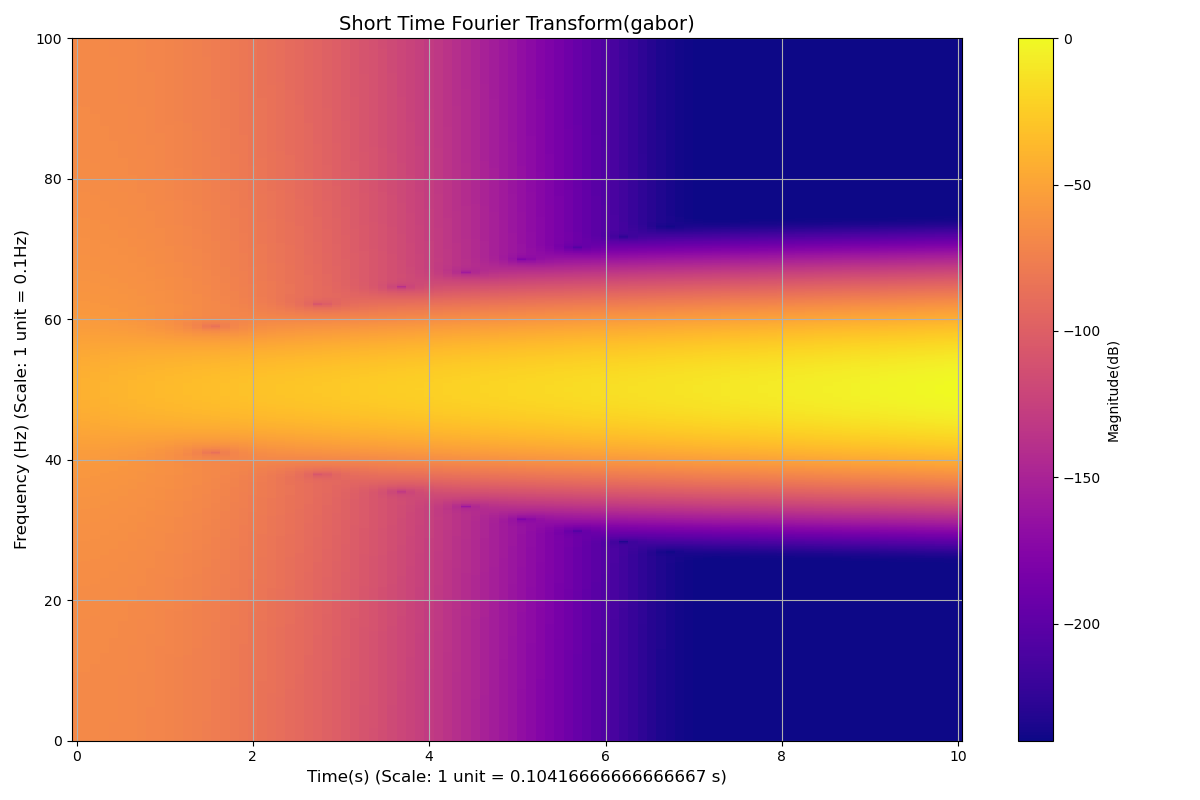
\includegraphics[scale = 0.35]{Gau_Win_gabor_21_250.0.png}
        \caption{STFT of $e^{-\frac{(x-5)^2}{\sigma^2}}sin(w_0t)$ with Window Size 250 and overlap of 229(Gaussian Window)}
        \label{fig:24}
        \end{figure}
    
    \end{itemize}

    In case of Bartlett Window, it is invertible as the sum of the windows is 1. We can take sample points of $S(t,\omega)$ at particular sample instants like $S(k\tau, \omega)$ and sum over those values, we would get the value of $f(t)$.    
    \item[(b)] \textbf{The Wigner-Ville Distribution:}
    With Wigner-Ville Distribution, the resolution is much sharper, specially in case of sin and linear chirp. Wigner Ville Distribution is invertible when the value of the conjugate of the function at 0 is not equal to 0. So, that is the case except for the first problem of $sin(w_ot)$. In all other cases, the function is invertible. The results of the wvd plot is given as follows: 

        \begin{figure}[H]
        \centering
        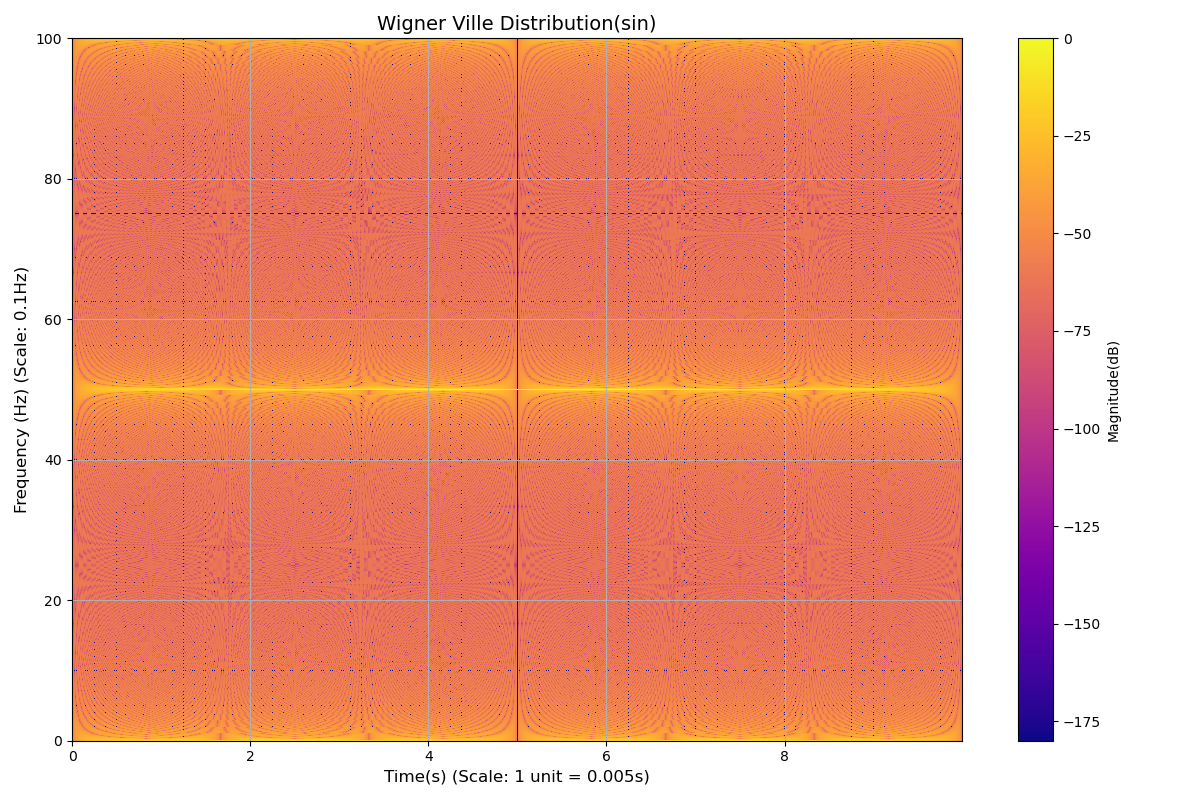
\includegraphics[scale = 0.35]{sin_wvd.png}
        \caption{WVD of $sin(w_0t)$}
        \label{fig:25}
        \end{figure}

        \begin{figure}[H]
        \centering
        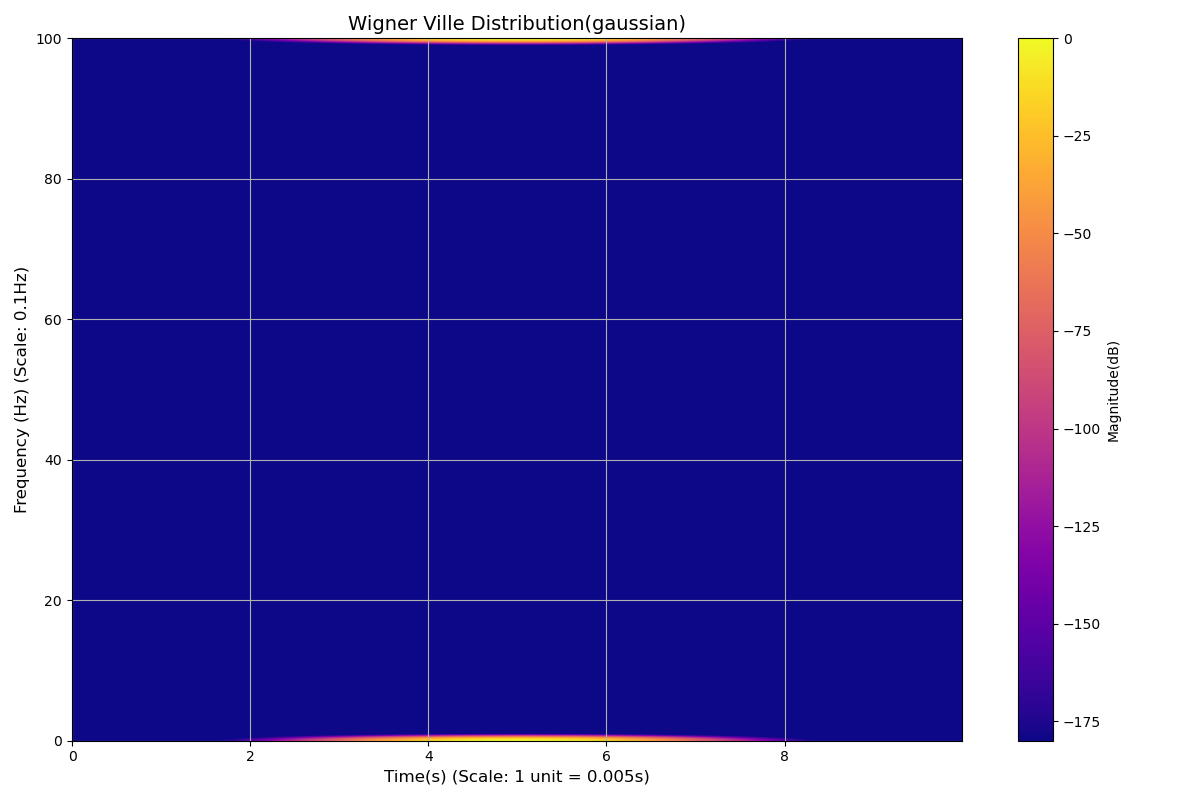
\includegraphics[scale = 0.35]{gaussian_wvd.png}
        \caption{WVD of $e^{-\frac{(x-5)^2}{\sigma^2}}$ }
        \label{fig:26}
        \end{figure}

        \begin{figure}[H]
        \centering
        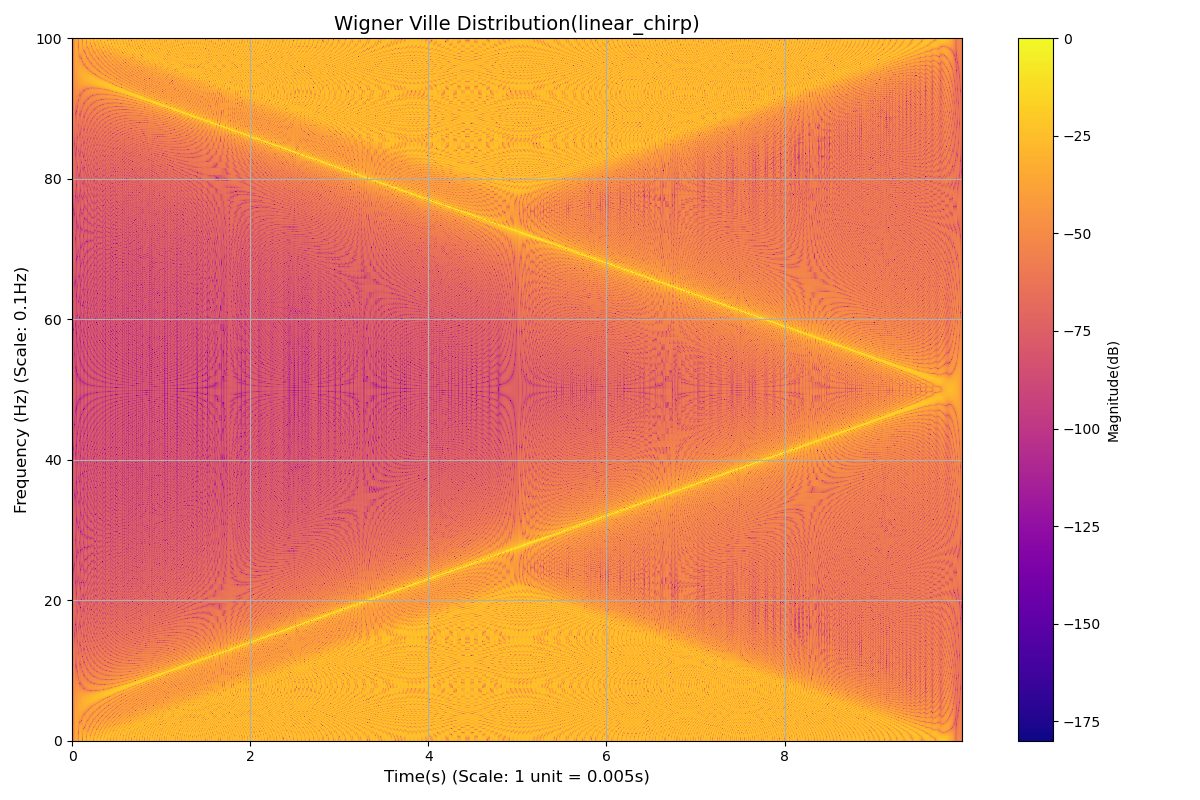
\includegraphics[scale = 0.35]{linear_chirp_wvd.png}
        \caption{WVD of $sin(2\pi\gamma(t)t)$, where $\gamma(t)$ varies linearly between $5Hz$ and $50Hz$}
        \label{fig:27}
        \end{figure}

        \begin{figure}[H]
        \centering
        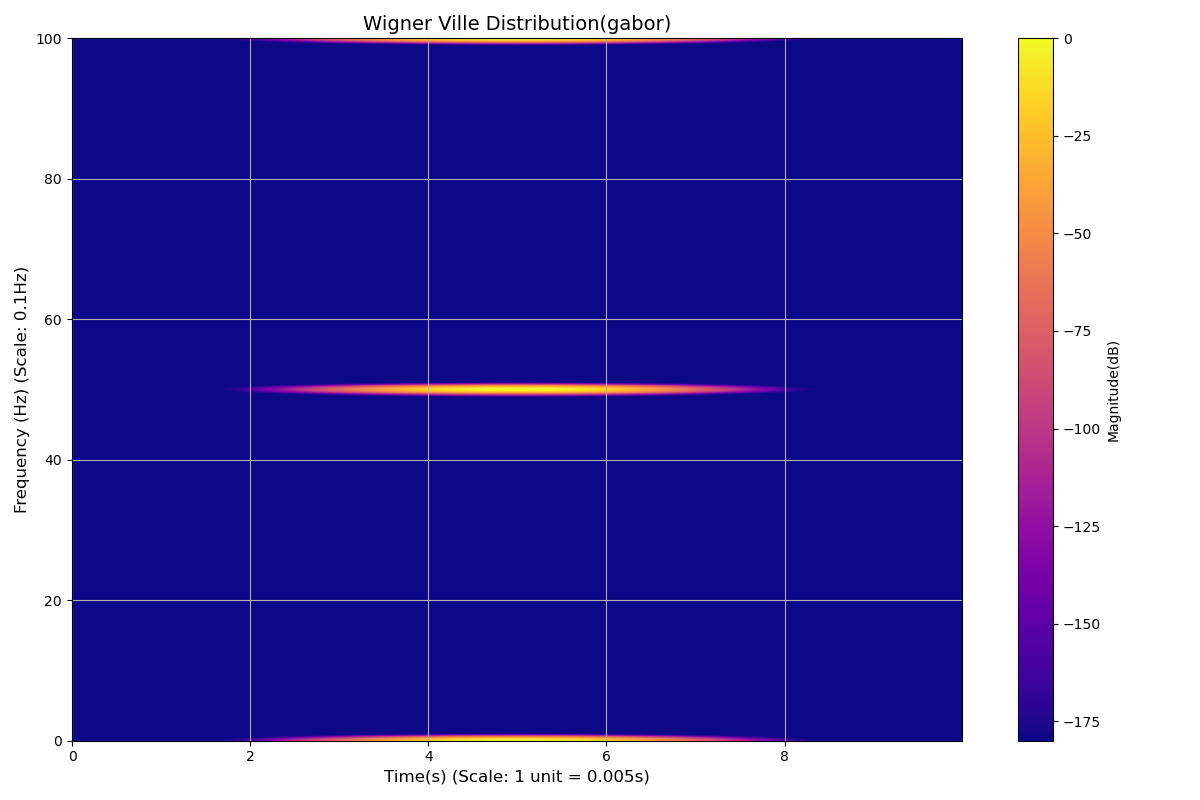
\includegraphics[scale = 0.35]{gabor_wvd.png}
        \caption{WVD of $e^{-\frac{(x-5)^2}{\sigma^2}}sin(w_0t)$}
        \label{fig:28}
        \end{figure}
  \end{itemize}
\end{solution}

\questionheader{2. STFT and PWVD for Real Life Signals}
\begin{solution}
  
  For large signals, the STFT and PWVD is done for chunks of data as processing of the whole signal at once was not possible with this computing power. There was no overlap kept between chunks due to lack of computation power. For that also some useful information may be lost while doing those STFT and WVD. For some data, the details seems to be missing due to performing this chunked STFT and PWVD. Also, in case of the music file, the first file consists of no data, so it is intentionally skipped. Same Bartlett window was used for all the case. Similar window is kept for both STFT and Pseudo WVD for suitable comparison

  \begin{itemize}
    \item[$\bullet$] EEG
  \end{itemize}
        \begin{figure}[H]
        \centering
        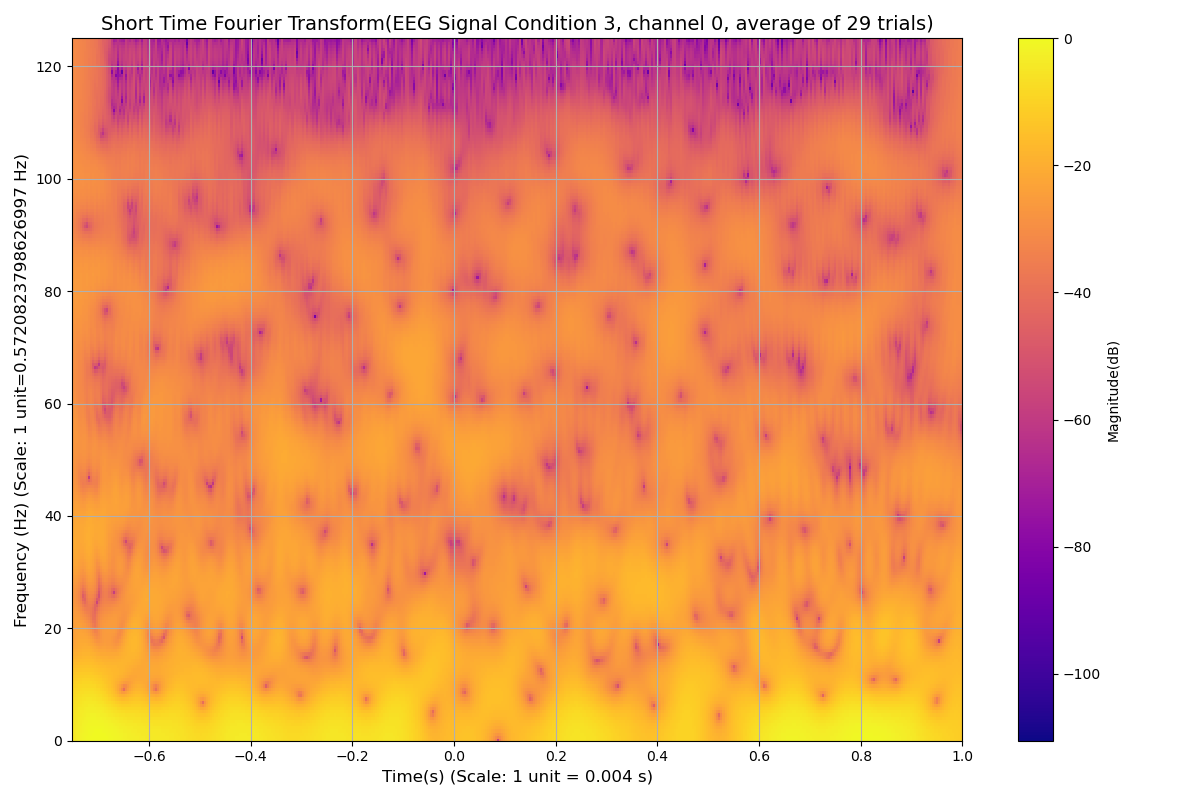
\includegraphics[scale = 0.35]{eegsignal_stft.png}
        \caption{STFT of EEG Signal for a particular case and a particular channel}
        \label{fig:29}
        \end{figure}

        \begin{figure}[H]
        \centering
        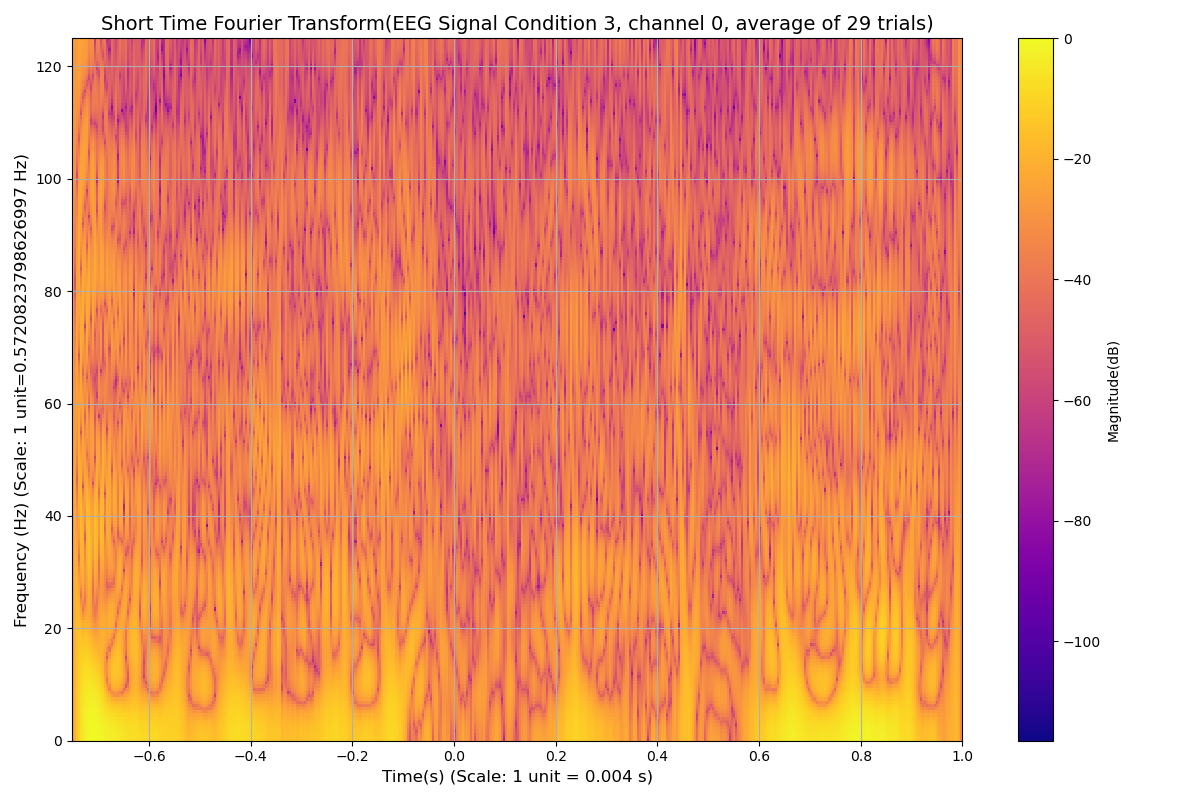
\includegraphics[scale = 0.35]{eegsignal_pwvd.png}
        \caption{Pseudo WVD of EEG Signal for a particular case and a particular channel}
        \label{fig:30}
        \end{figure}    

  \begin{itemize}
    \item[$\bullet$] LIGO
  \end{itemize}
        \begin{figure}[H]
        \centering
        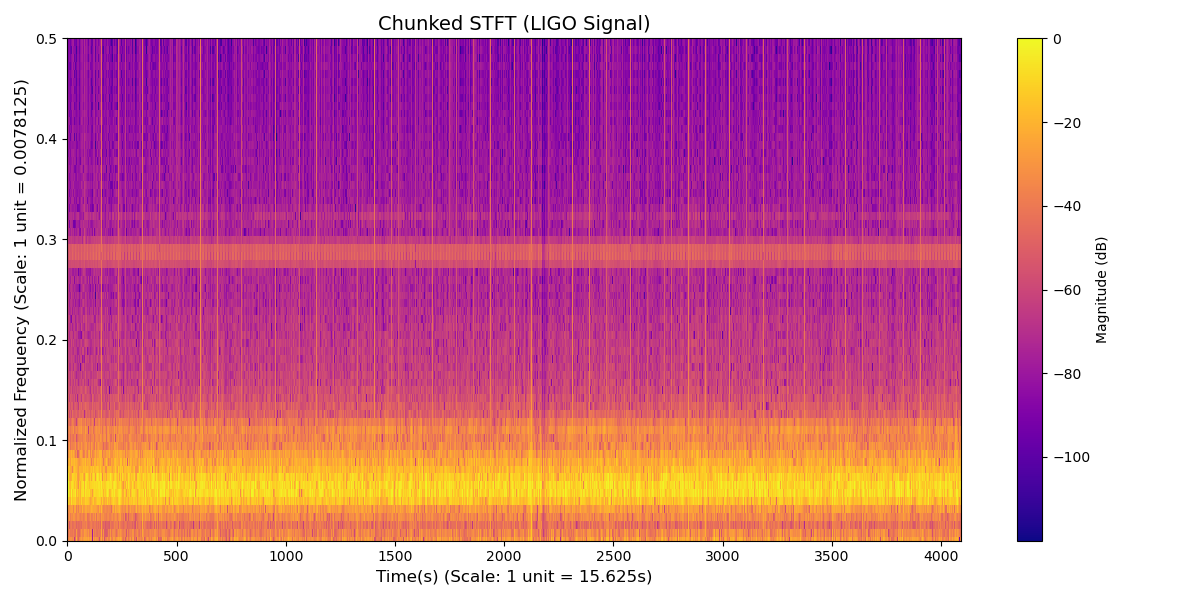
\includegraphics[scale = 0.45]{ligosignal_stft.png}
        \caption{STFT of for LIGO Signal}
        \label{fig:31}
        \end{figure}

        \begin{figure}[H]
        \centering
        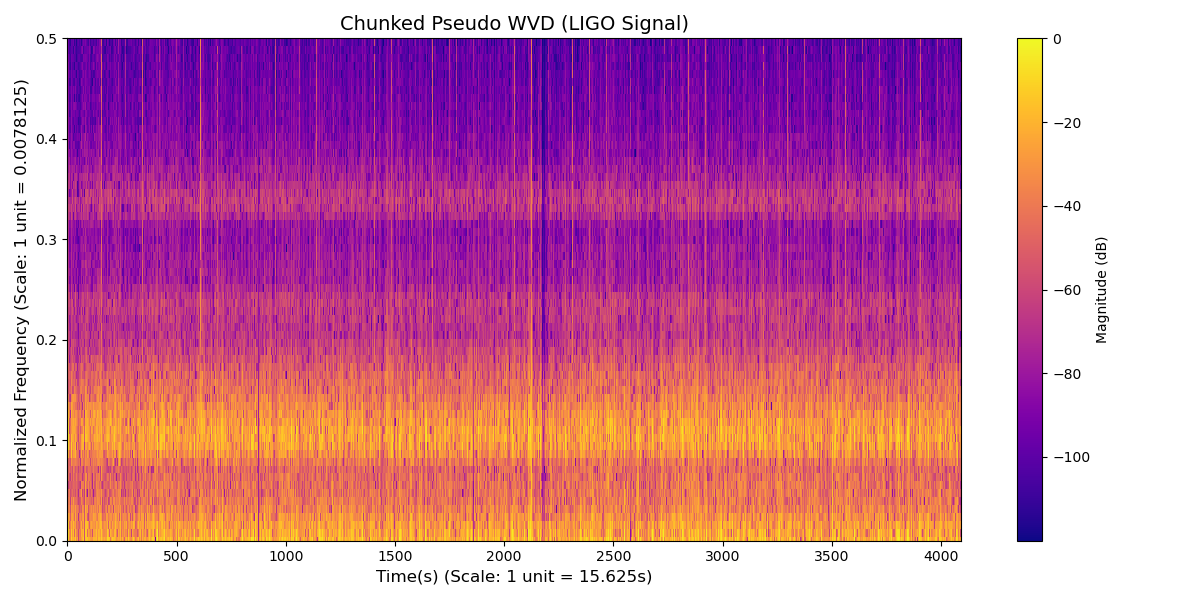
\includegraphics[scale = 0.45]{ligosignal_pwvd.png}
        \caption{Pseudo WVD of for LIGO Signal}
        \label{fig:32}
        \end{figure}   

  \begin{itemize}
    \item[$\bullet$] mmWave Radar
  \end{itemize}

        \begin{figure}[H]
        \centering
        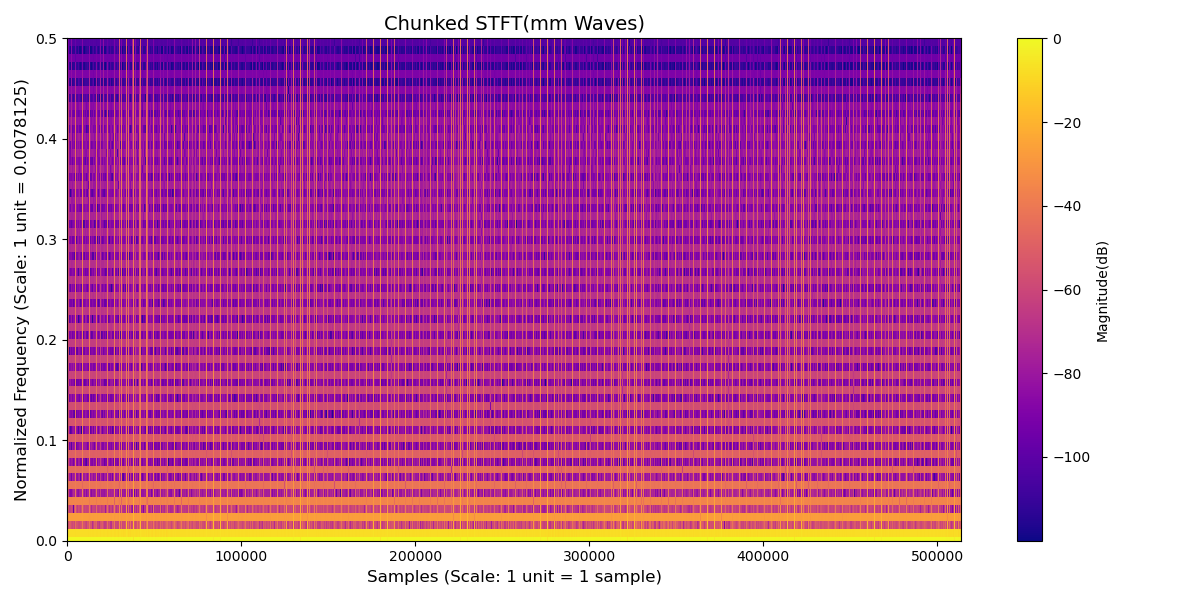
\includegraphics[scale = 0.45]{mmWaves_stft.png}
        \caption{STFT of MmWave Radar Signal}
        \label{fig:33}
        \end{figure}

        \begin{figure}[H]
        \centering
        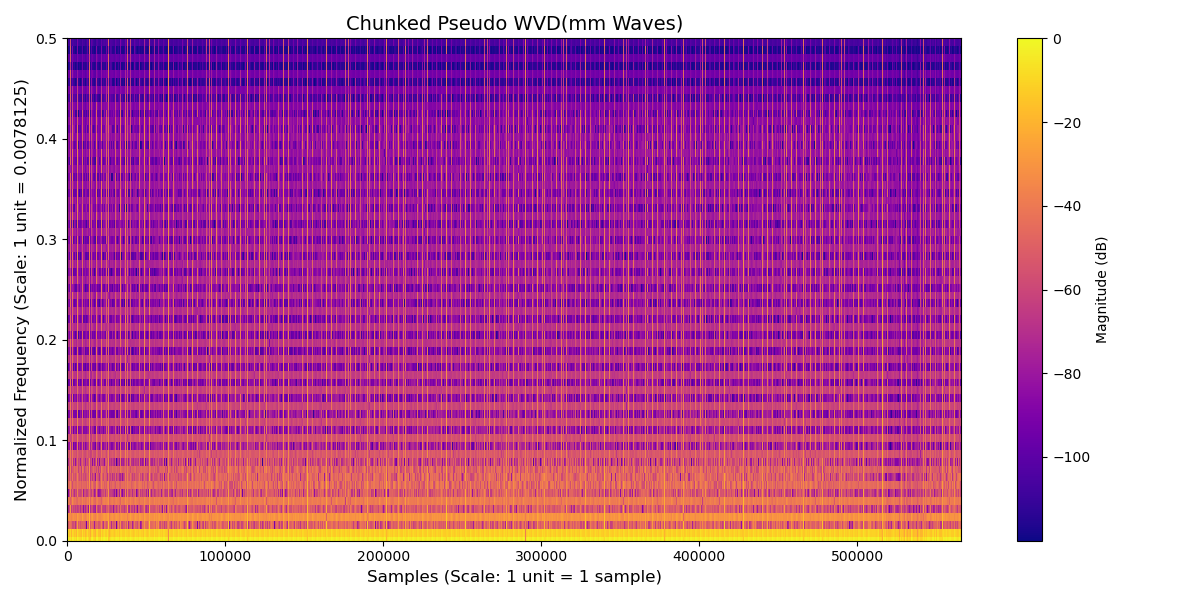
\includegraphics[scale = 0.45]{mmWaves_pwvd.png}
        \caption{Pseudo WVD of MmWave Radar Signal}
        \label{fig:34}
        \end{figure}    

  \begin{itemize}
    \item[$\bullet$] Music Fig.\ref{fig:35} - Fig.\ref{fig:40} shows the STFT plots and Fig.\ref{fig:41} - Fig.\ref{fig:46} shows the PWVD of the music files. The white gaps in the plots is for the zones where there is no value of the muusic, i.e. there is no music. 
  \end{itemize}
        \begin{figure}[H]
        \centering
        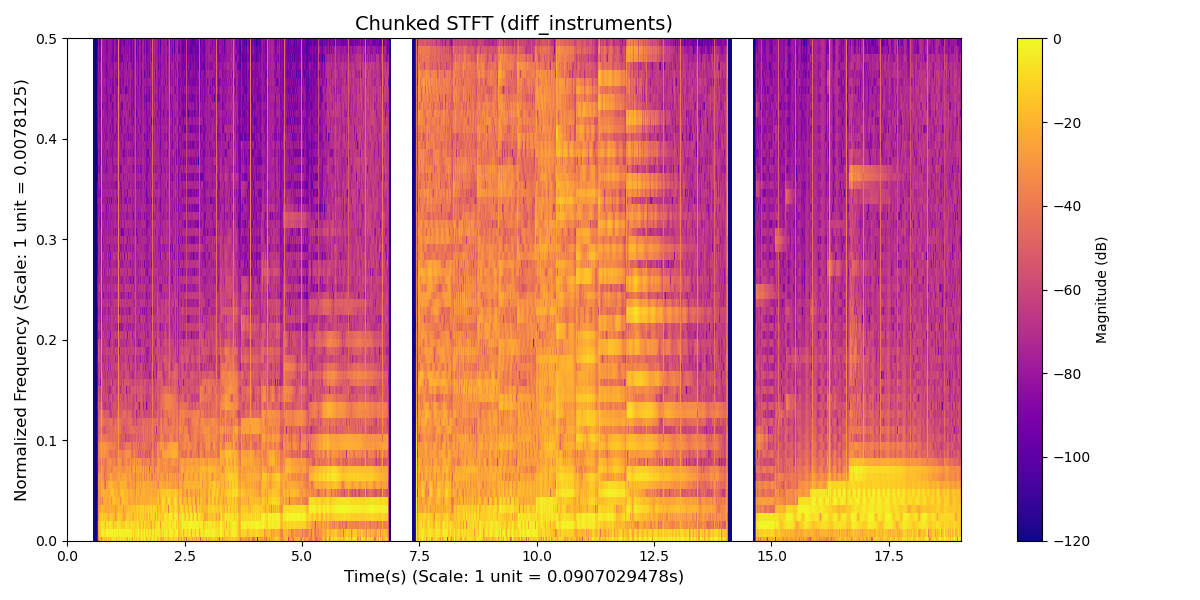
\includegraphics[scale = 0.45]{music_diff_instruments_stft.png}
        \caption{STFT of Music(Diff Instruments)}
        \label{fig:35}
        \end{figure}

        \begin{figure}[H]
        \centering
        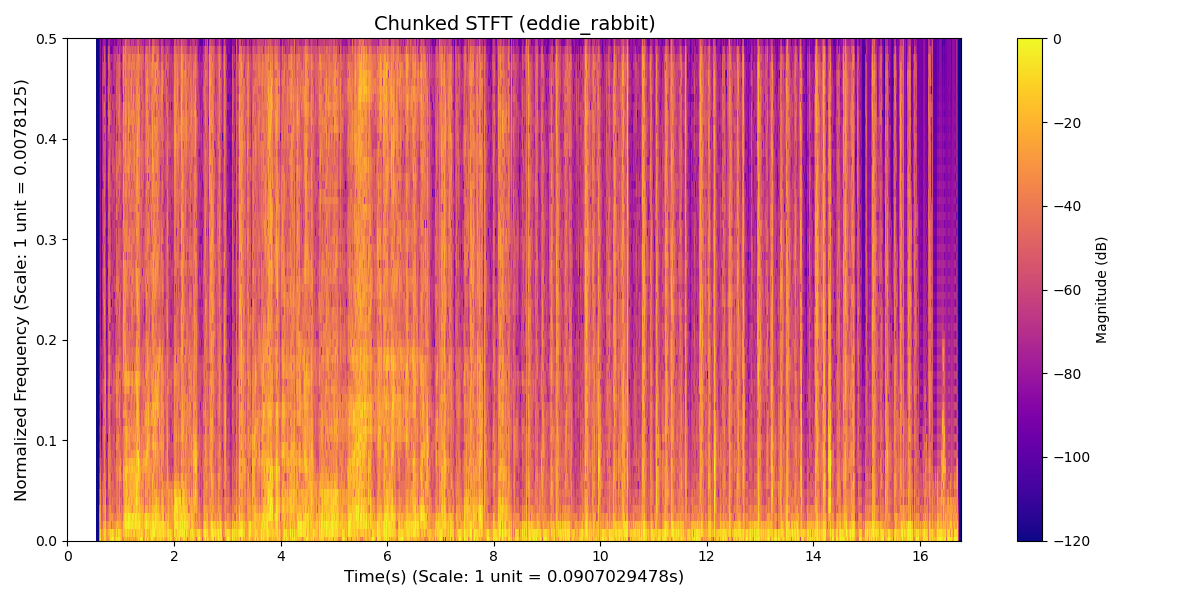
\includegraphics[scale = 0.45]{music_eddie_rabbit_stft.png}
        \caption{STFT of Music(Eddie Rabbit)}
        \label{fig:36}
        \end{figure}

        \begin{figure}[H]
        \centering
        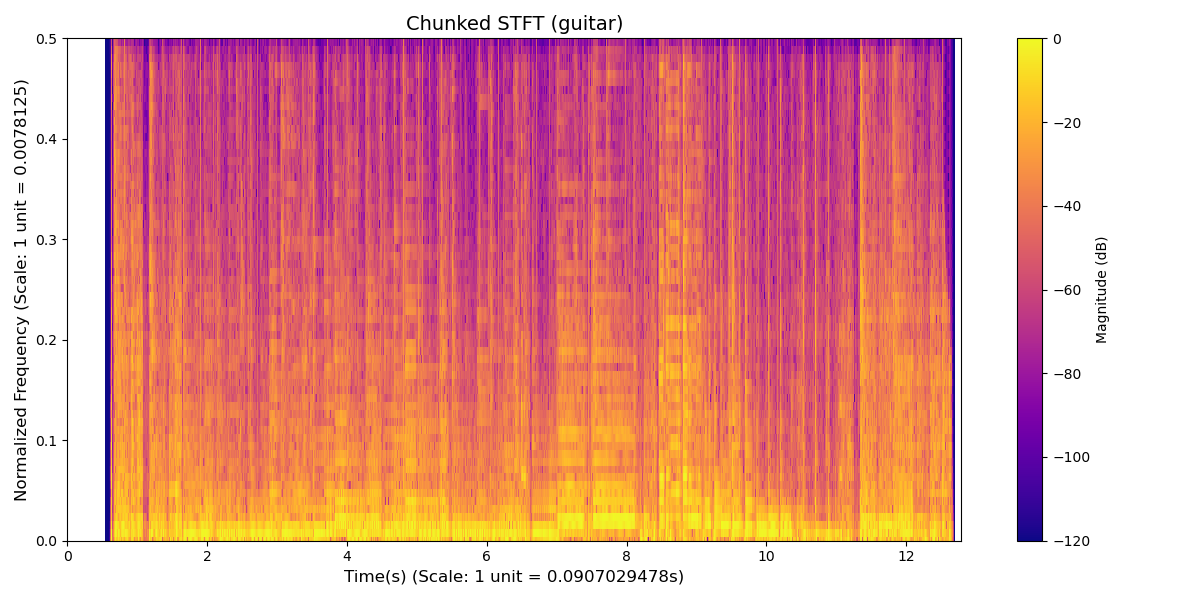
\includegraphics[scale = 0.45]{music_guitar_stft.png}
        \caption{STFT of Music(Guitar)}
        \label{fig:37}
        \end{figure}

        \begin{figure}[H]
        \centering
        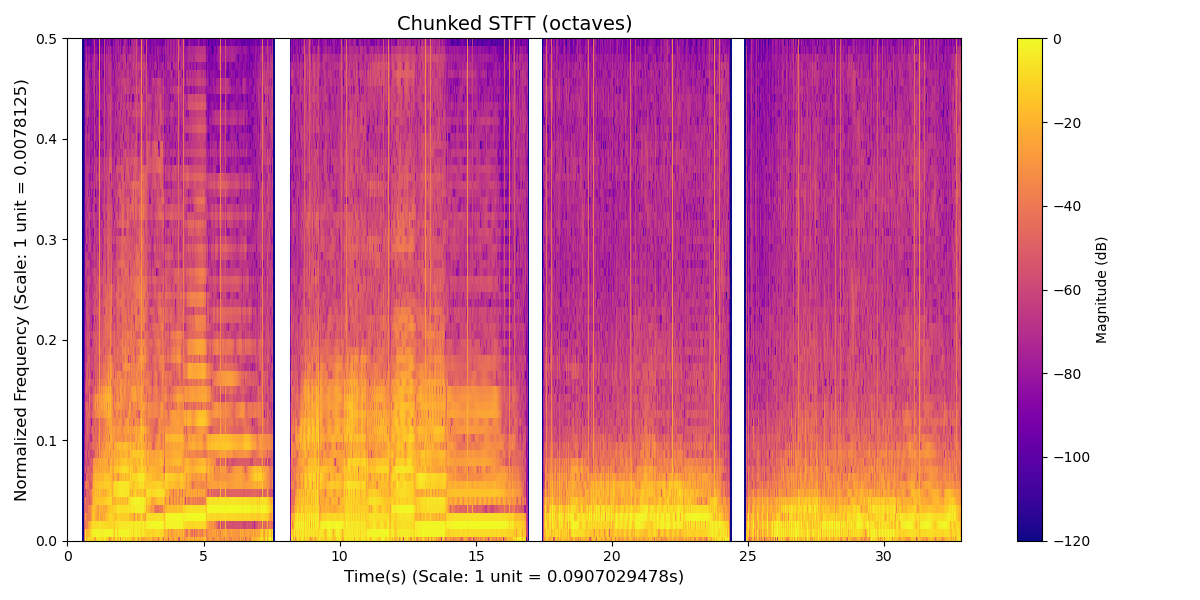
\includegraphics[scale = 0.45]{music_octaves_stft.png}
        \caption{STFT of Music(Octaves)}
        \label{fig:38}
        \end{figure}

        \begin{figure}[H]
        \centering
        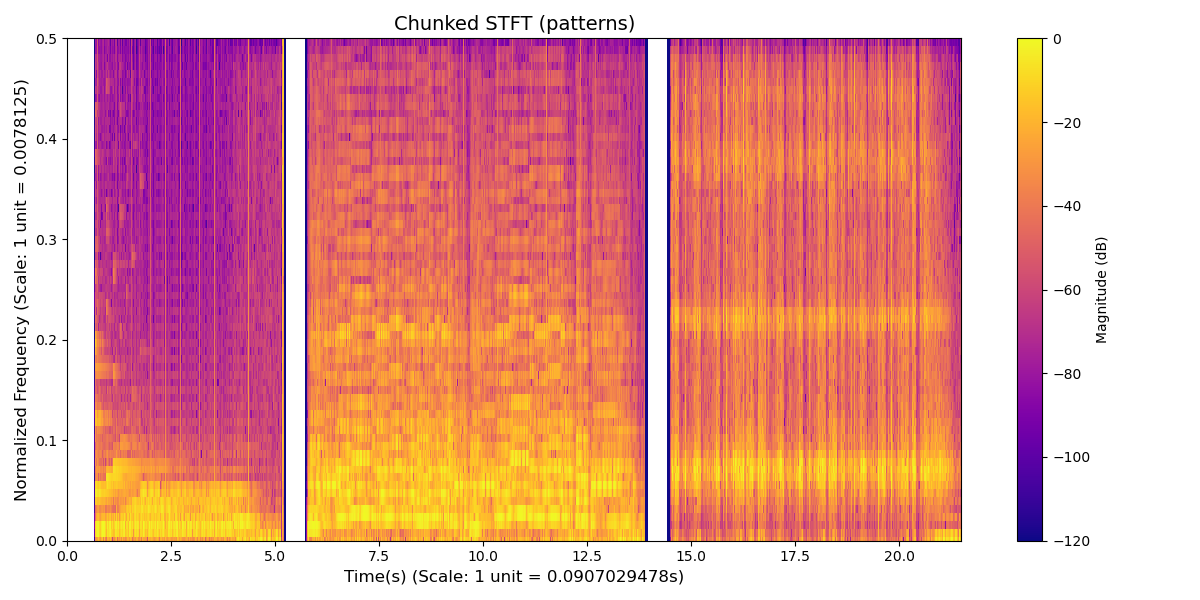
\includegraphics[scale = 0.45]{music_patterns_stft.png}
        \caption{STFT of Music(Patterns)}
        \label{fig:39}
        \end{figure}

        \begin{figure}[H]
        \centering
        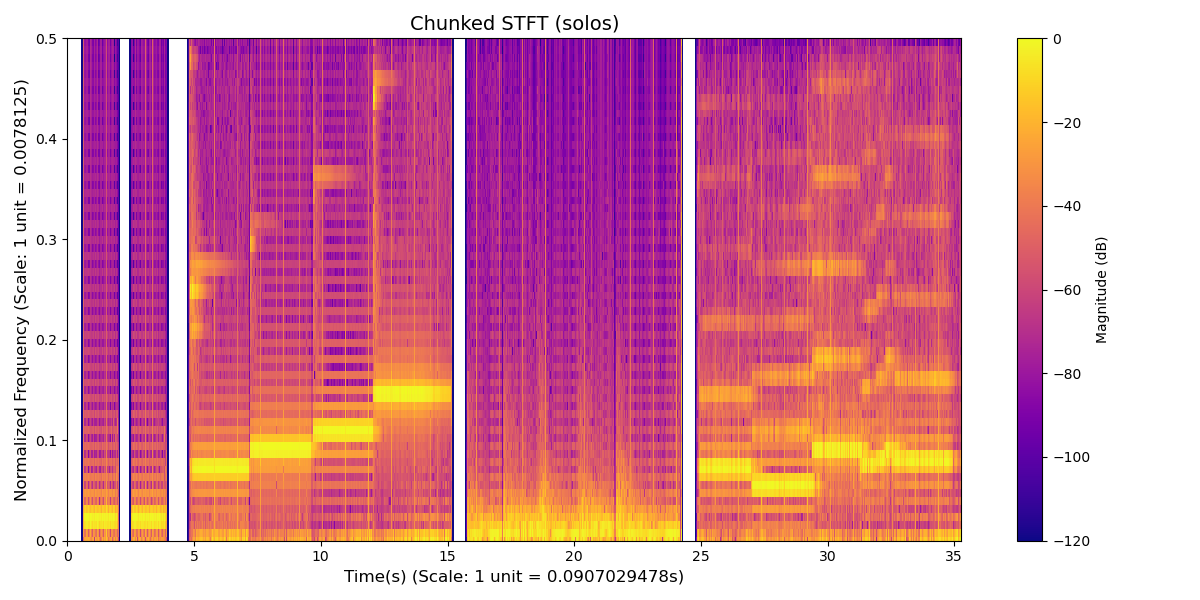
\includegraphics[scale = 0.45]{music_solos_stft.png}
        \caption{STFT of Music(Solos)}
        \label{fig:40}
        \end{figure}

        \begin{figure}[H]
        \centering
        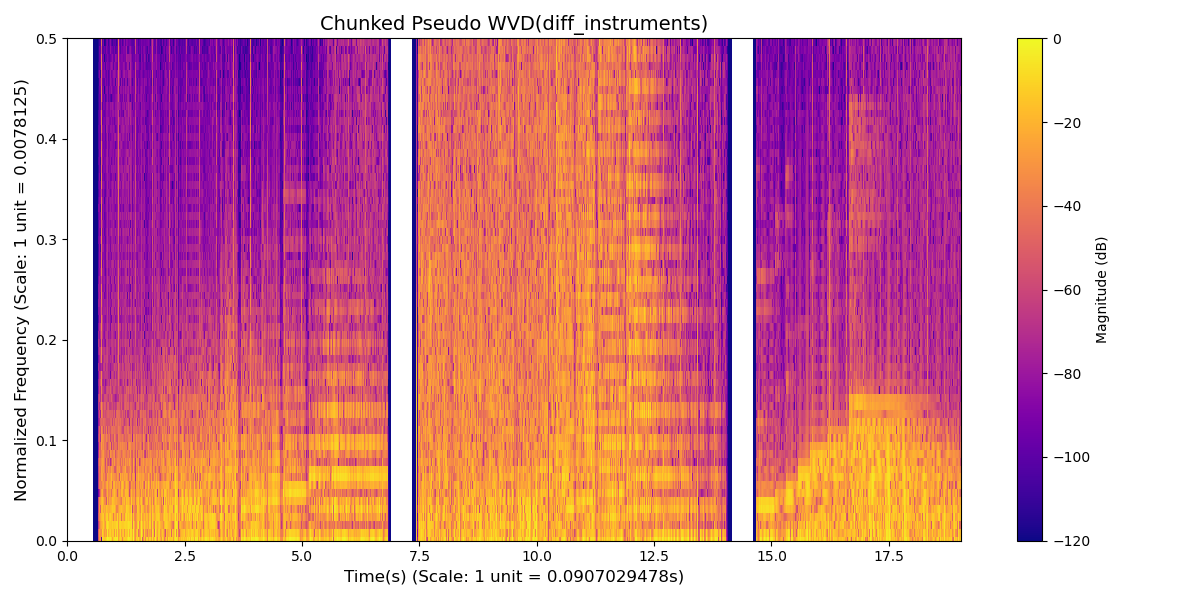
\includegraphics[scale = 0.45]{music_diff_instruments_pwvd.png}
        \caption{Pseudo WVD of Music(Diff Instruments)}
        \label{fig:41}
        \end{figure}    

        \begin{figure}[H]
        \centering
        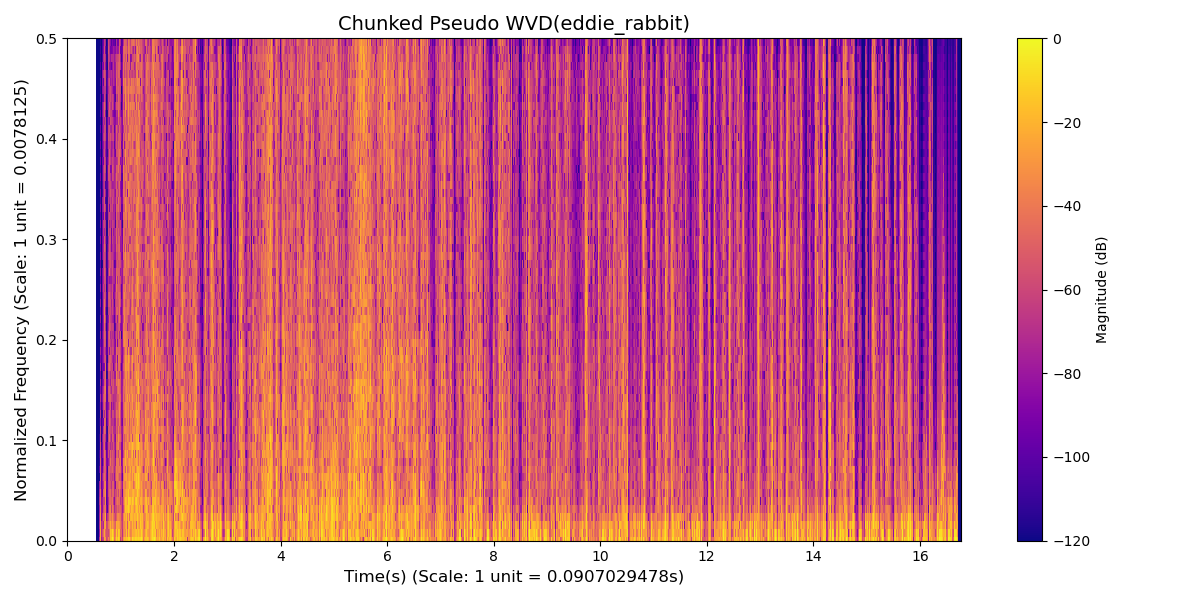
\includegraphics[scale = 0.45]{music_eddie_rabbit_pwvd.png}
        \caption{Pseudo WVD of Music(Eddie Rabbit)}
        \label{fig:42}
        \end{figure}    

        \begin{figure}[H]
        \centering
        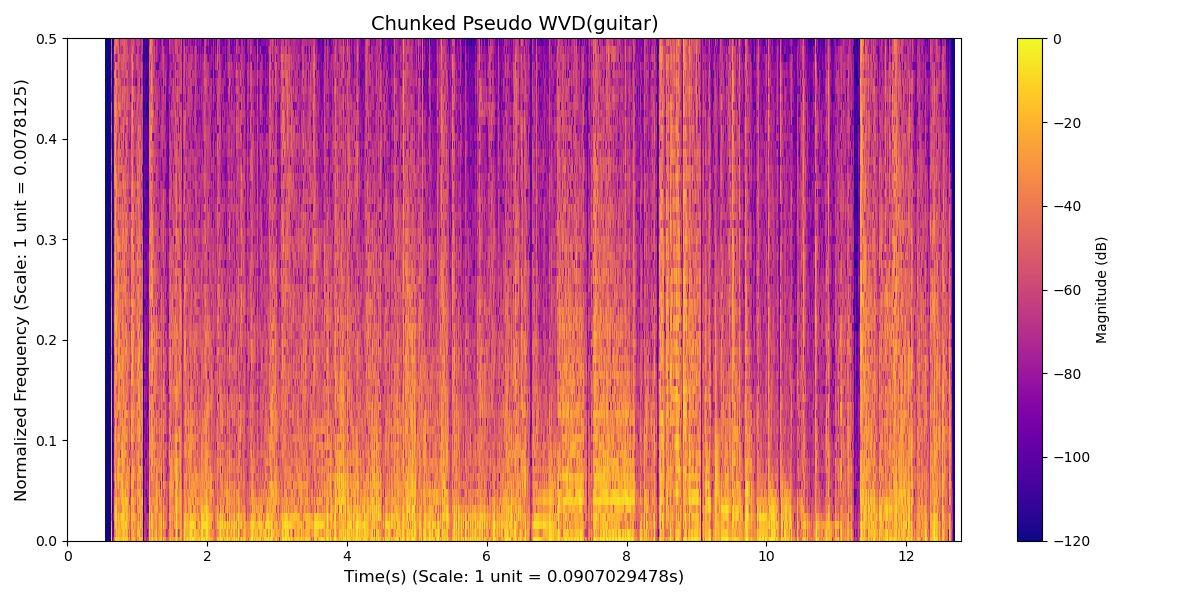
\includegraphics[scale = 0.45]{music_guitar_pwvd.png}
        \caption{Pseudo WVD of Music(Guitar)}
        \label{fig:43}
        \end{figure}    

        \begin{figure}[H]
        \centering
        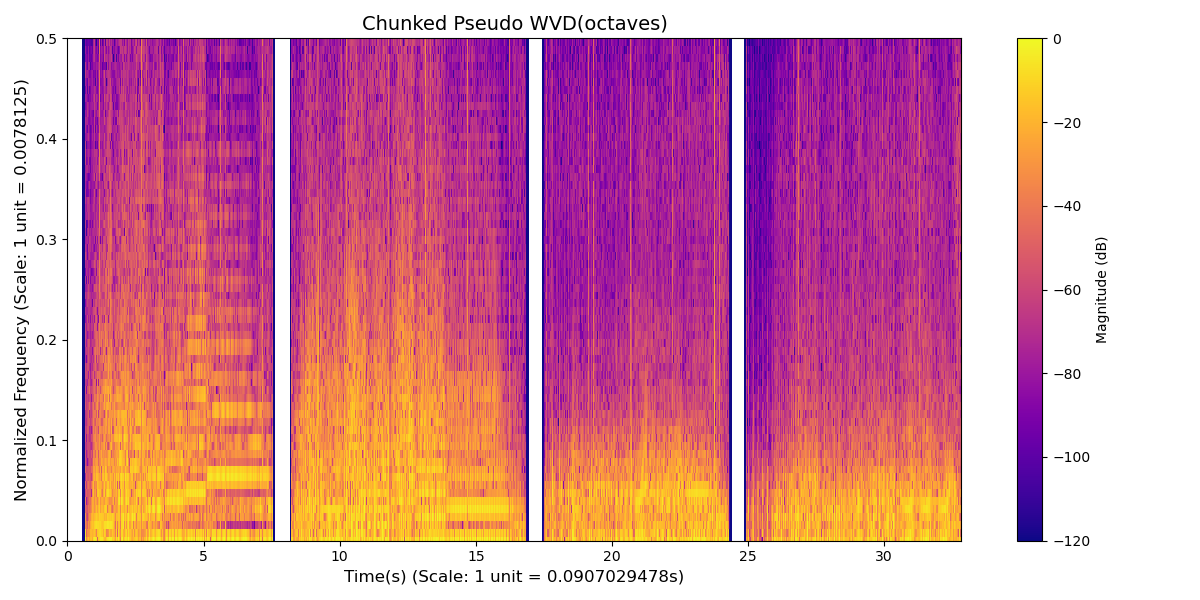
\includegraphics[scale = 0.45]{music_octaves_pwvd.png}
        \caption{Pseudo WVD of Music(Octaves)}
        \label{fig:44}
        \end{figure}    

        \begin{figure}[H]
        \centering
        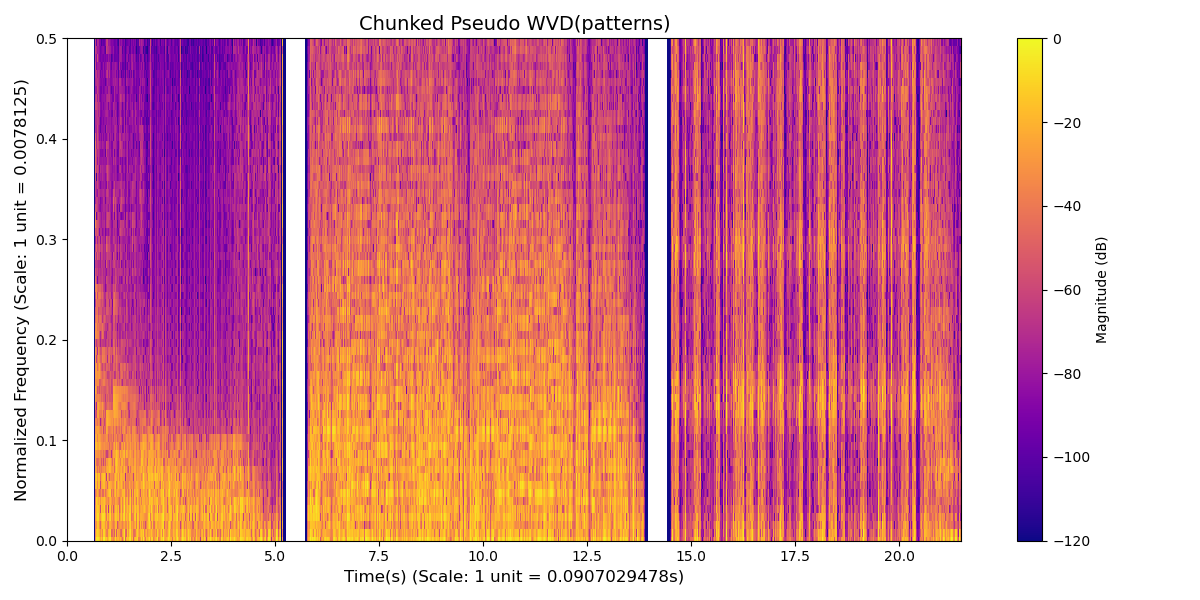
\includegraphics[scale = 0.45]{music_patterns_pwvd.png}
        \caption{Pseudo WVD of Music(Patterns)}
        \label{fig:45}
        \end{figure}   

        \begin{figure}[H]
        \centering
        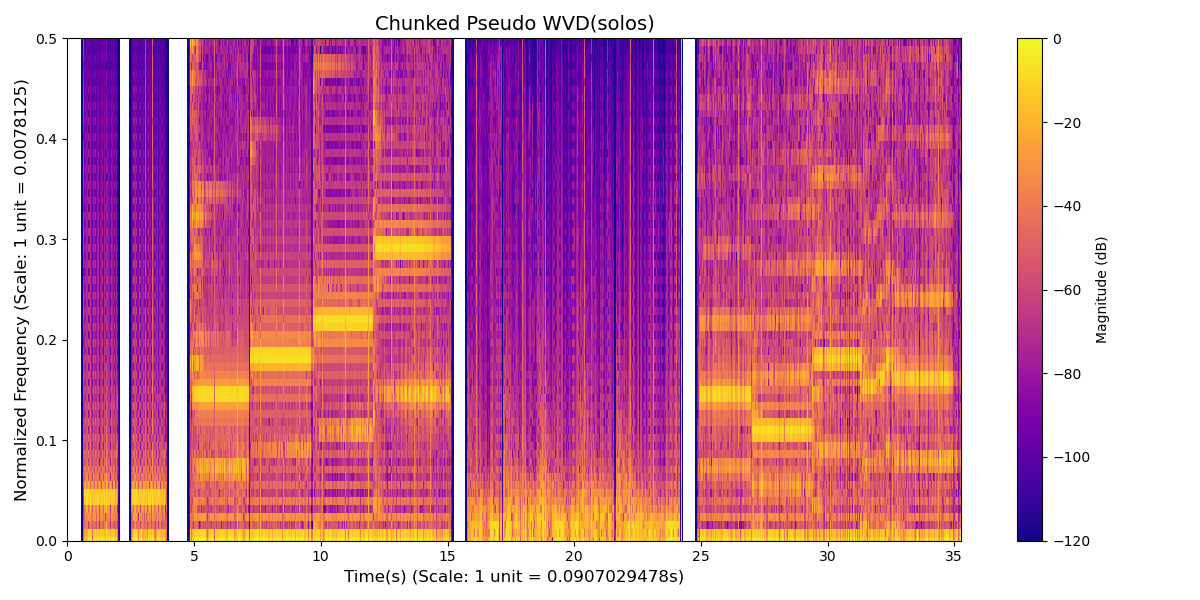
\includegraphics[scale = 0.45]{music_solos_pwvd.png}
        \caption{Pseudo WVD of Music(Solos)}
        \label{fig:46}
        \end{figure}    

      \begin{itemize}
      \item[$\bullet$] Radar Demo
      \end{itemize}

        \begin{figure}[H]
        \centering
        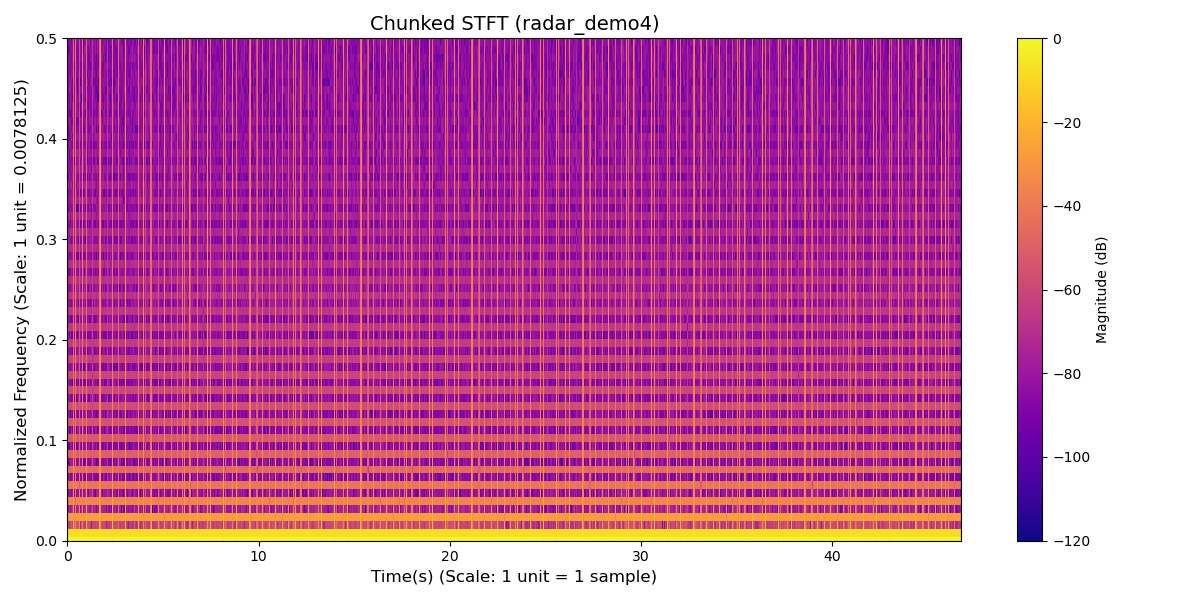
\includegraphics[scale = 0.45]{radar_demo4_stft.png}
        \caption{STFT of Radar Demo 4}
        \label{fig:47}
        \end{figure}

        \begin{figure}[H]
        \centering
        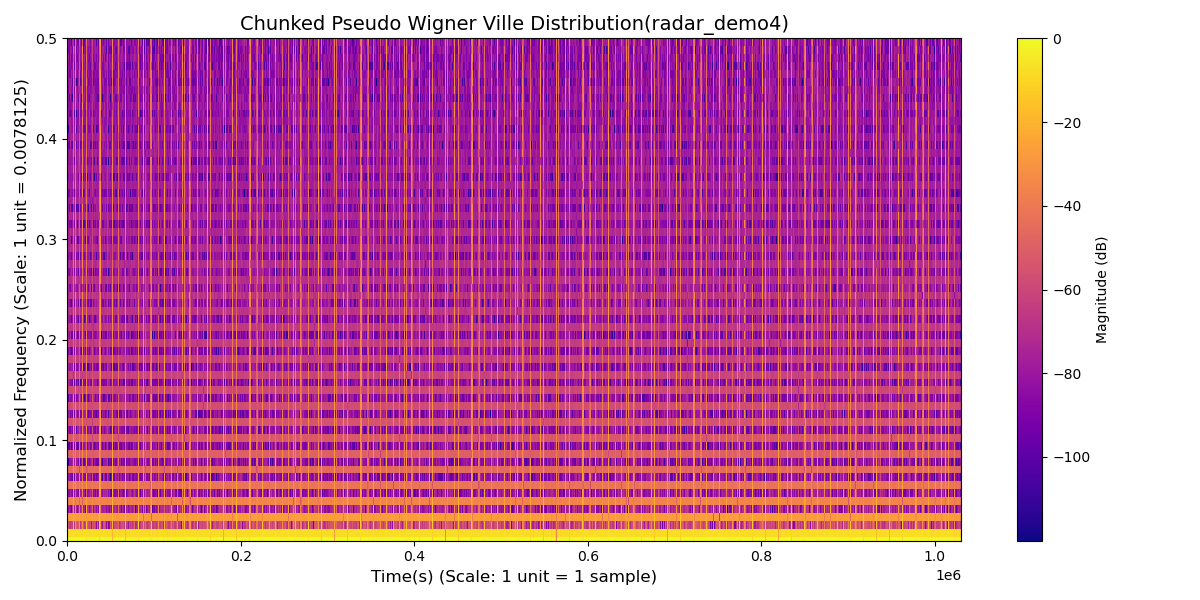
\includegraphics[scale = 0.45]{radar_demo4_pwvd.png}
        \caption{Pseudo WVD of Radar Demo 4}
        \label{fig:48}
        \end{figure}    

        \begin{figure}[H]
        \centering
        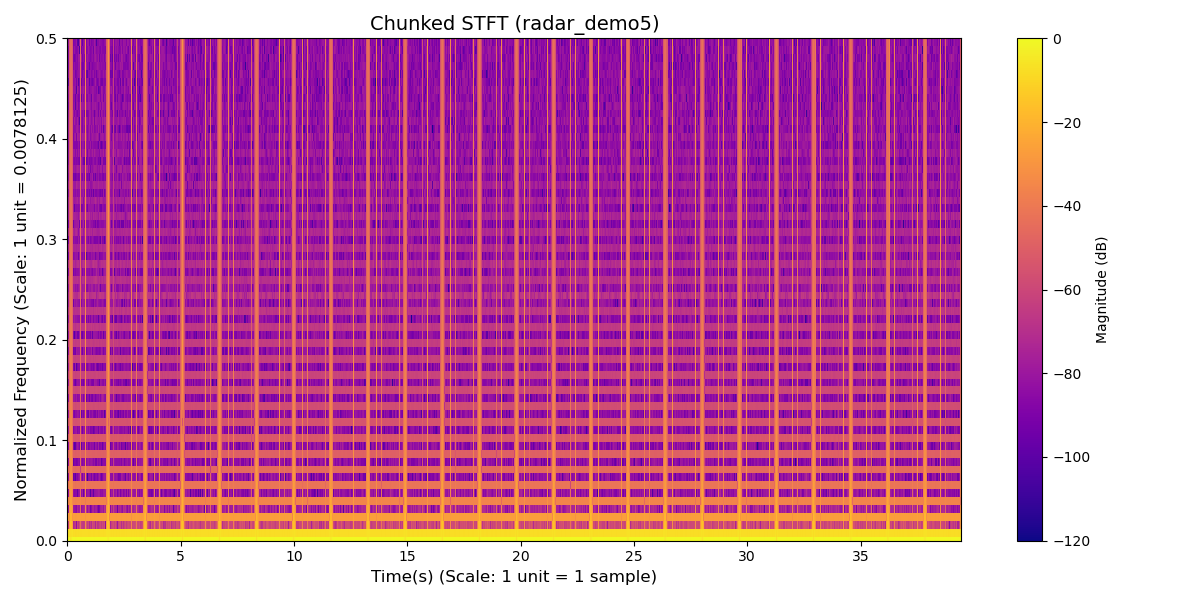
\includegraphics[scale = 0.45]{radar_demo5_stft.png}
        \caption{STFT of Radar Demo 5}
        \label{fig:49}
        \end{figure}

        \begin{figure}[H]
        \centering
        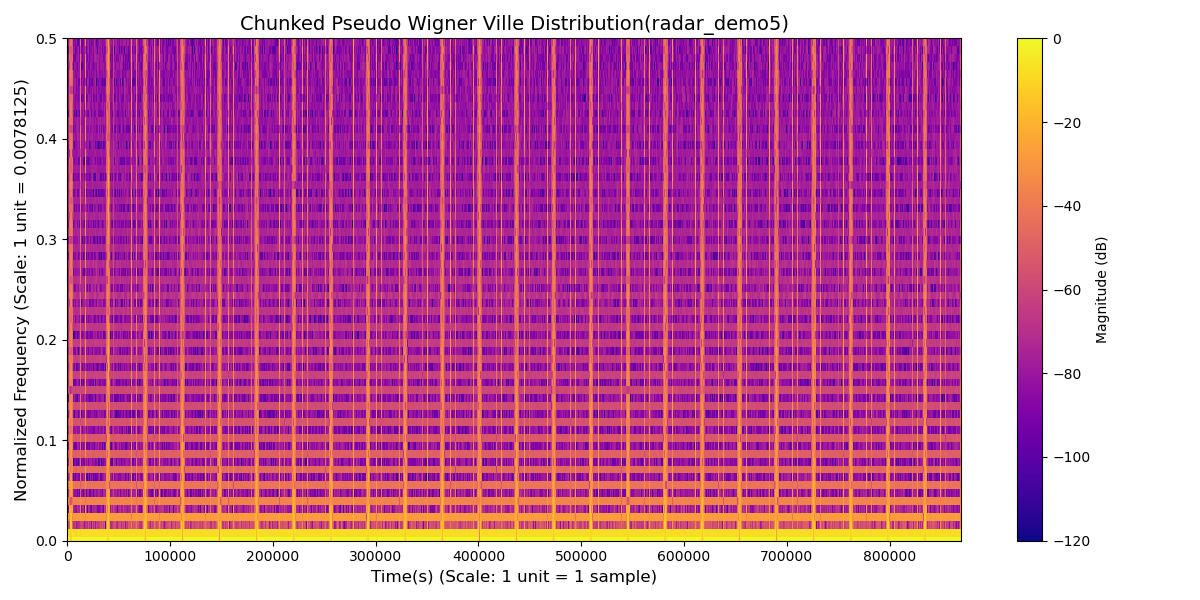
\includegraphics[scale = 0.45]{radar_demo5_pwvd.png}
        \caption{Pseudo WVD of Radar Demo 5}
        \label{fig:50}
        \end{figure}    

      \begin{itemize}
      \item[$\bullet$] Timit Speech
      \end{itemize}

        \begin{figure}[H]
        \centering
        \includegraphics[scale = 0.35]{timit_sa1_stft.png}
        \caption{STFT of Timit Sa1 Signal}
        \label{fig:51}
        \end{figure}

        \begin{figure}[H]
        \centering
        \includegraphics[scale = 0.35]{timit_sa1_pwvd.png}
        \caption{Pseudo WVD of Timit Sa1 Signal}
        \label{fig:52}
        \end{figure}      

        \begin{figure}[H]
        \centering
        \includegraphics[scale = 0.35]{timit_sa2_stft.png}
        \caption{STFT of Timit Sa2 Signal}
        \label{fig:53}
        \end{figure}

        \begin{figure}[H]
        \centering
        \includegraphics[scale = 0.35]{timit_sa2_pwvd.png}
        \caption{Pseudo WVD of Timit Sa2 Signal}
        \label{fig:54}
        \end{figure}      

        \begin{figure}[H]
        \centering
        \includegraphics[scale = 0.35]{timit_sx204_stft.png}
        \caption{STFT of Timit Sx204 Signal}
        \label{fig:55}
        \end{figure}

        \begin{figure}[H]
        \centering
        \includegraphics[scale = 0.35]{timit_sx204_pwvd.png}
        \caption{Pseudo WVD of Timit Sx204 Signal}
        \label{fig:56}
        \end{figure}      
  
\end{solution}

\end{document}